\subsection{SHAP analysis of general models}

%%%%%%%%%%% Discharge disability 0-2 %%%%%%%%%%%%%%%

%% All patients

\begin{figure}[htbp]
    \centering
    
    % Top image (Full width)
    \begin{subfigure}{0.50\textwidth}
        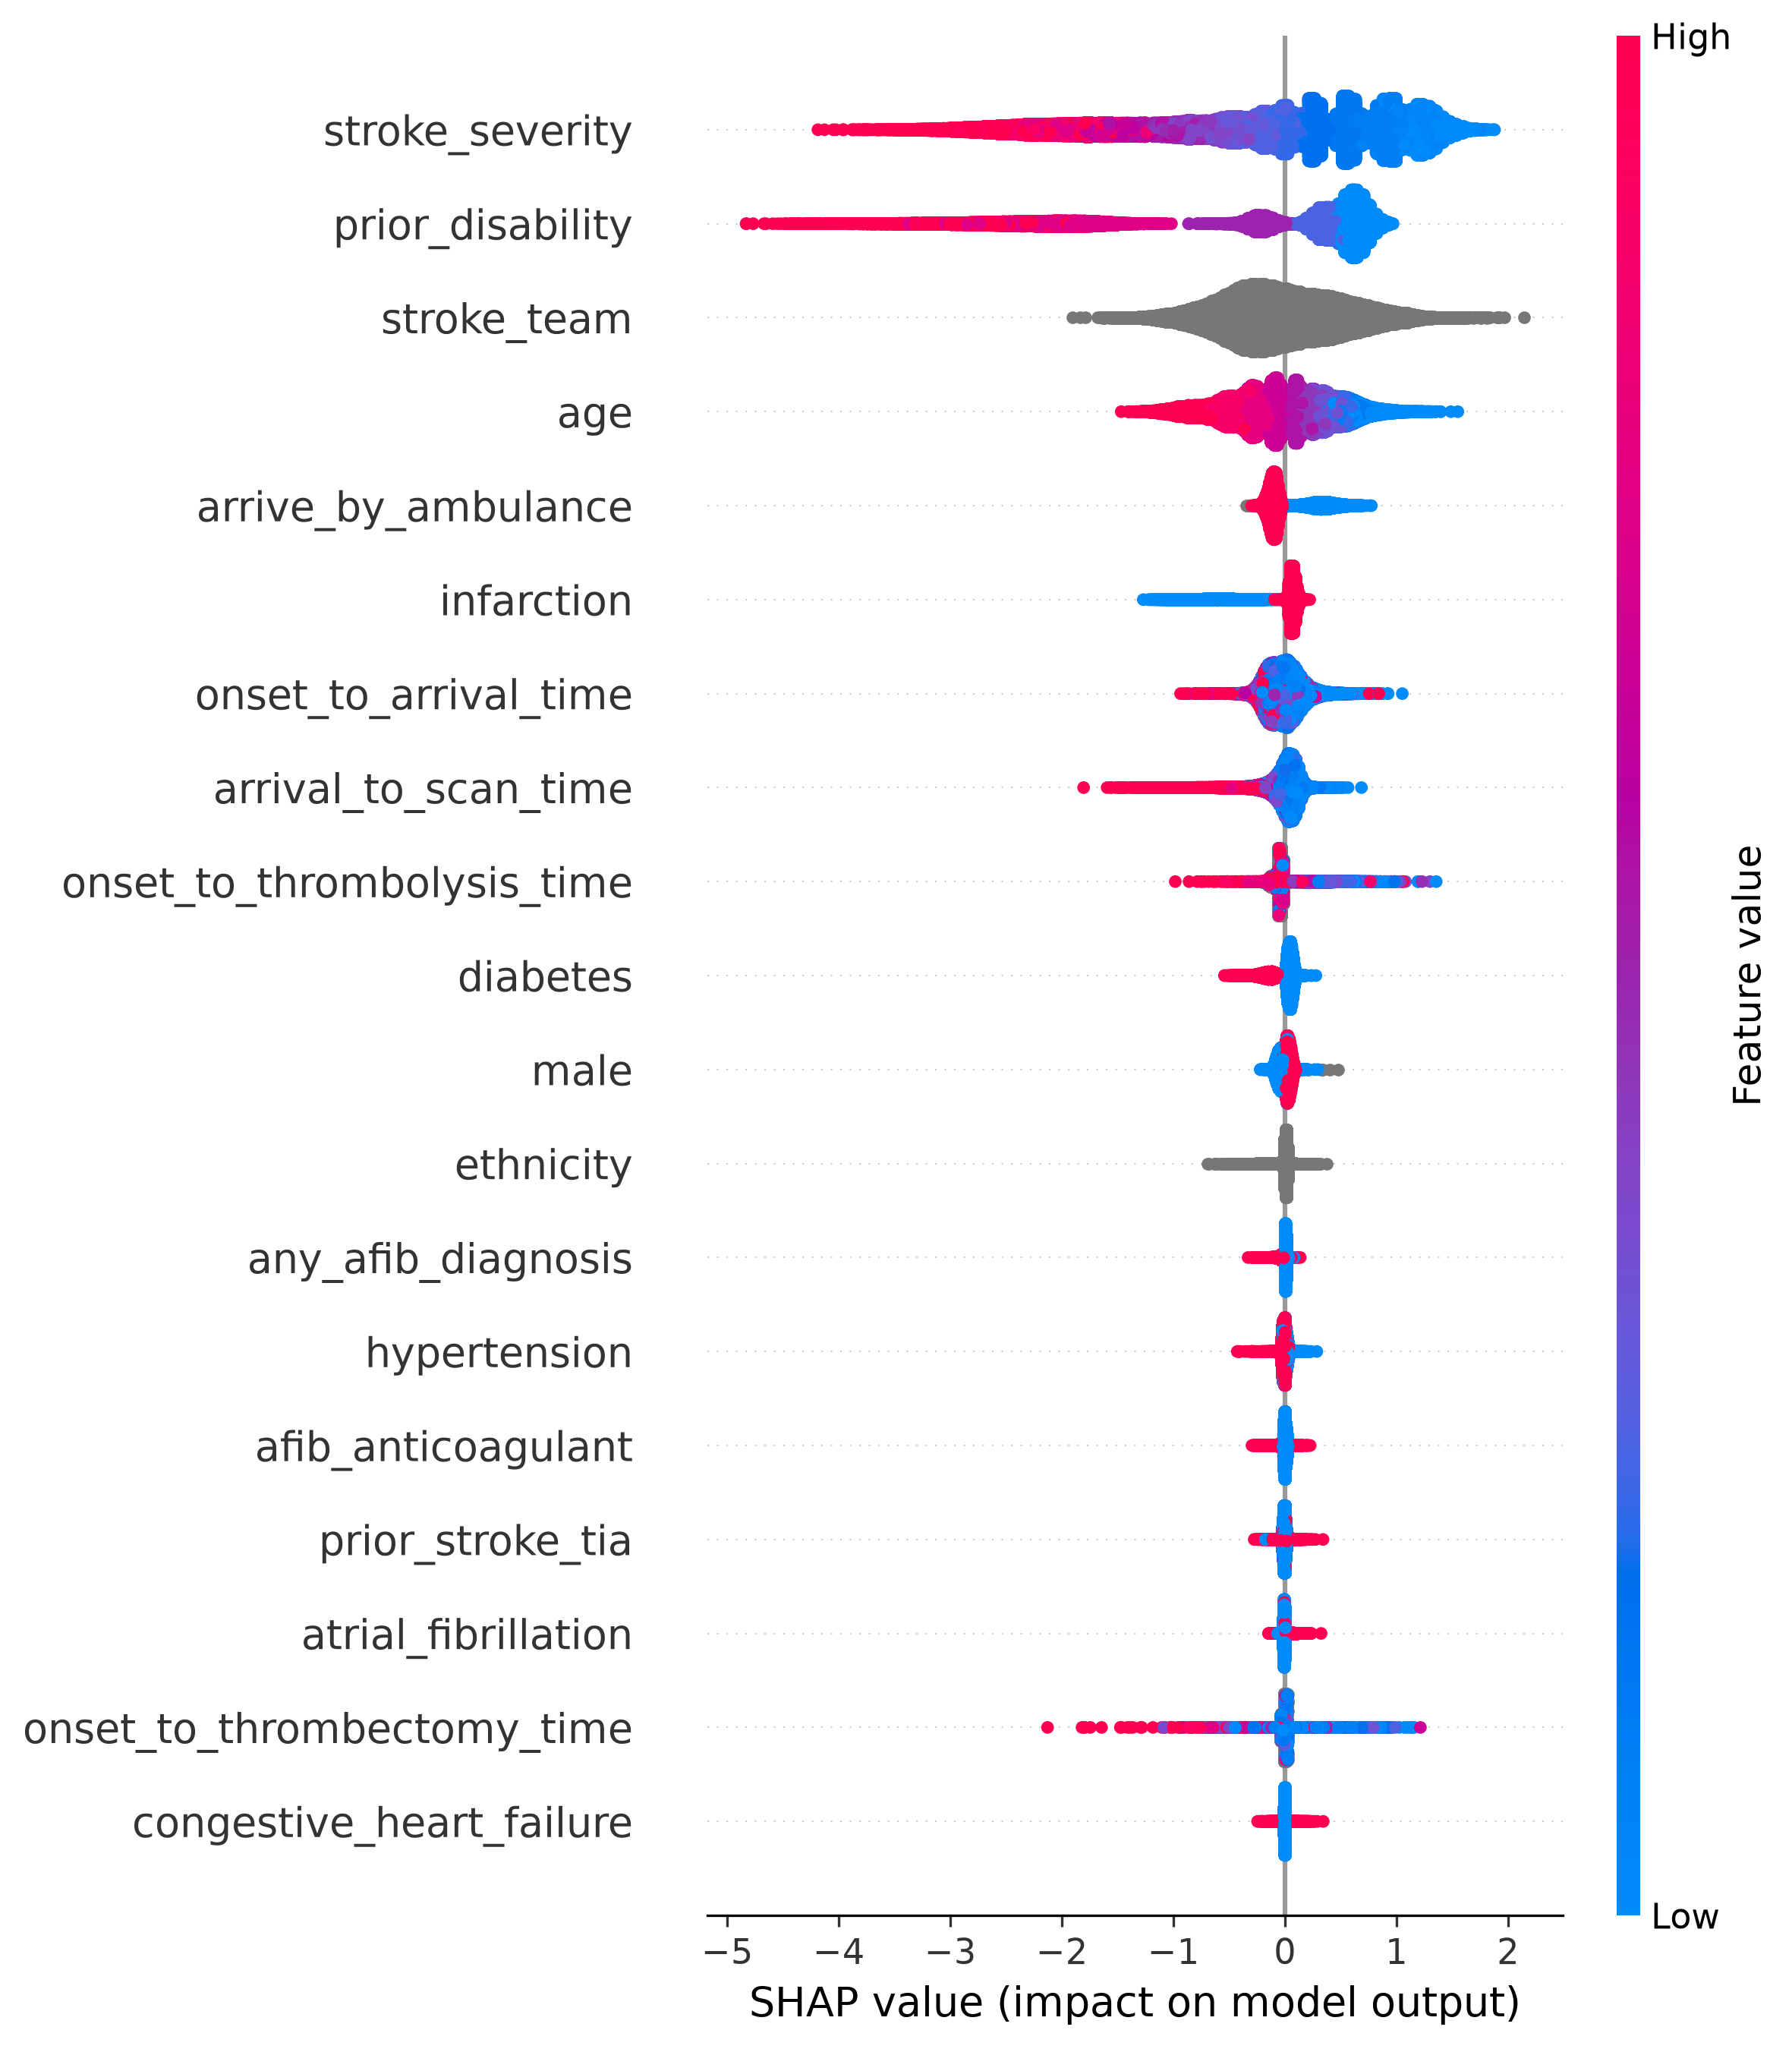
\includegraphics[width=\linewidth]{images/shap/shap_all_patients_mrs_less_than_3.png}
        %\caption{}
        \label{fig:top}
    \end{subfigure}

    \vspace{0.5cm} % Optional vertical space between rows

    % Bottom left image (~45% width)
    \begin{subfigure}{0.407\textwidth}
        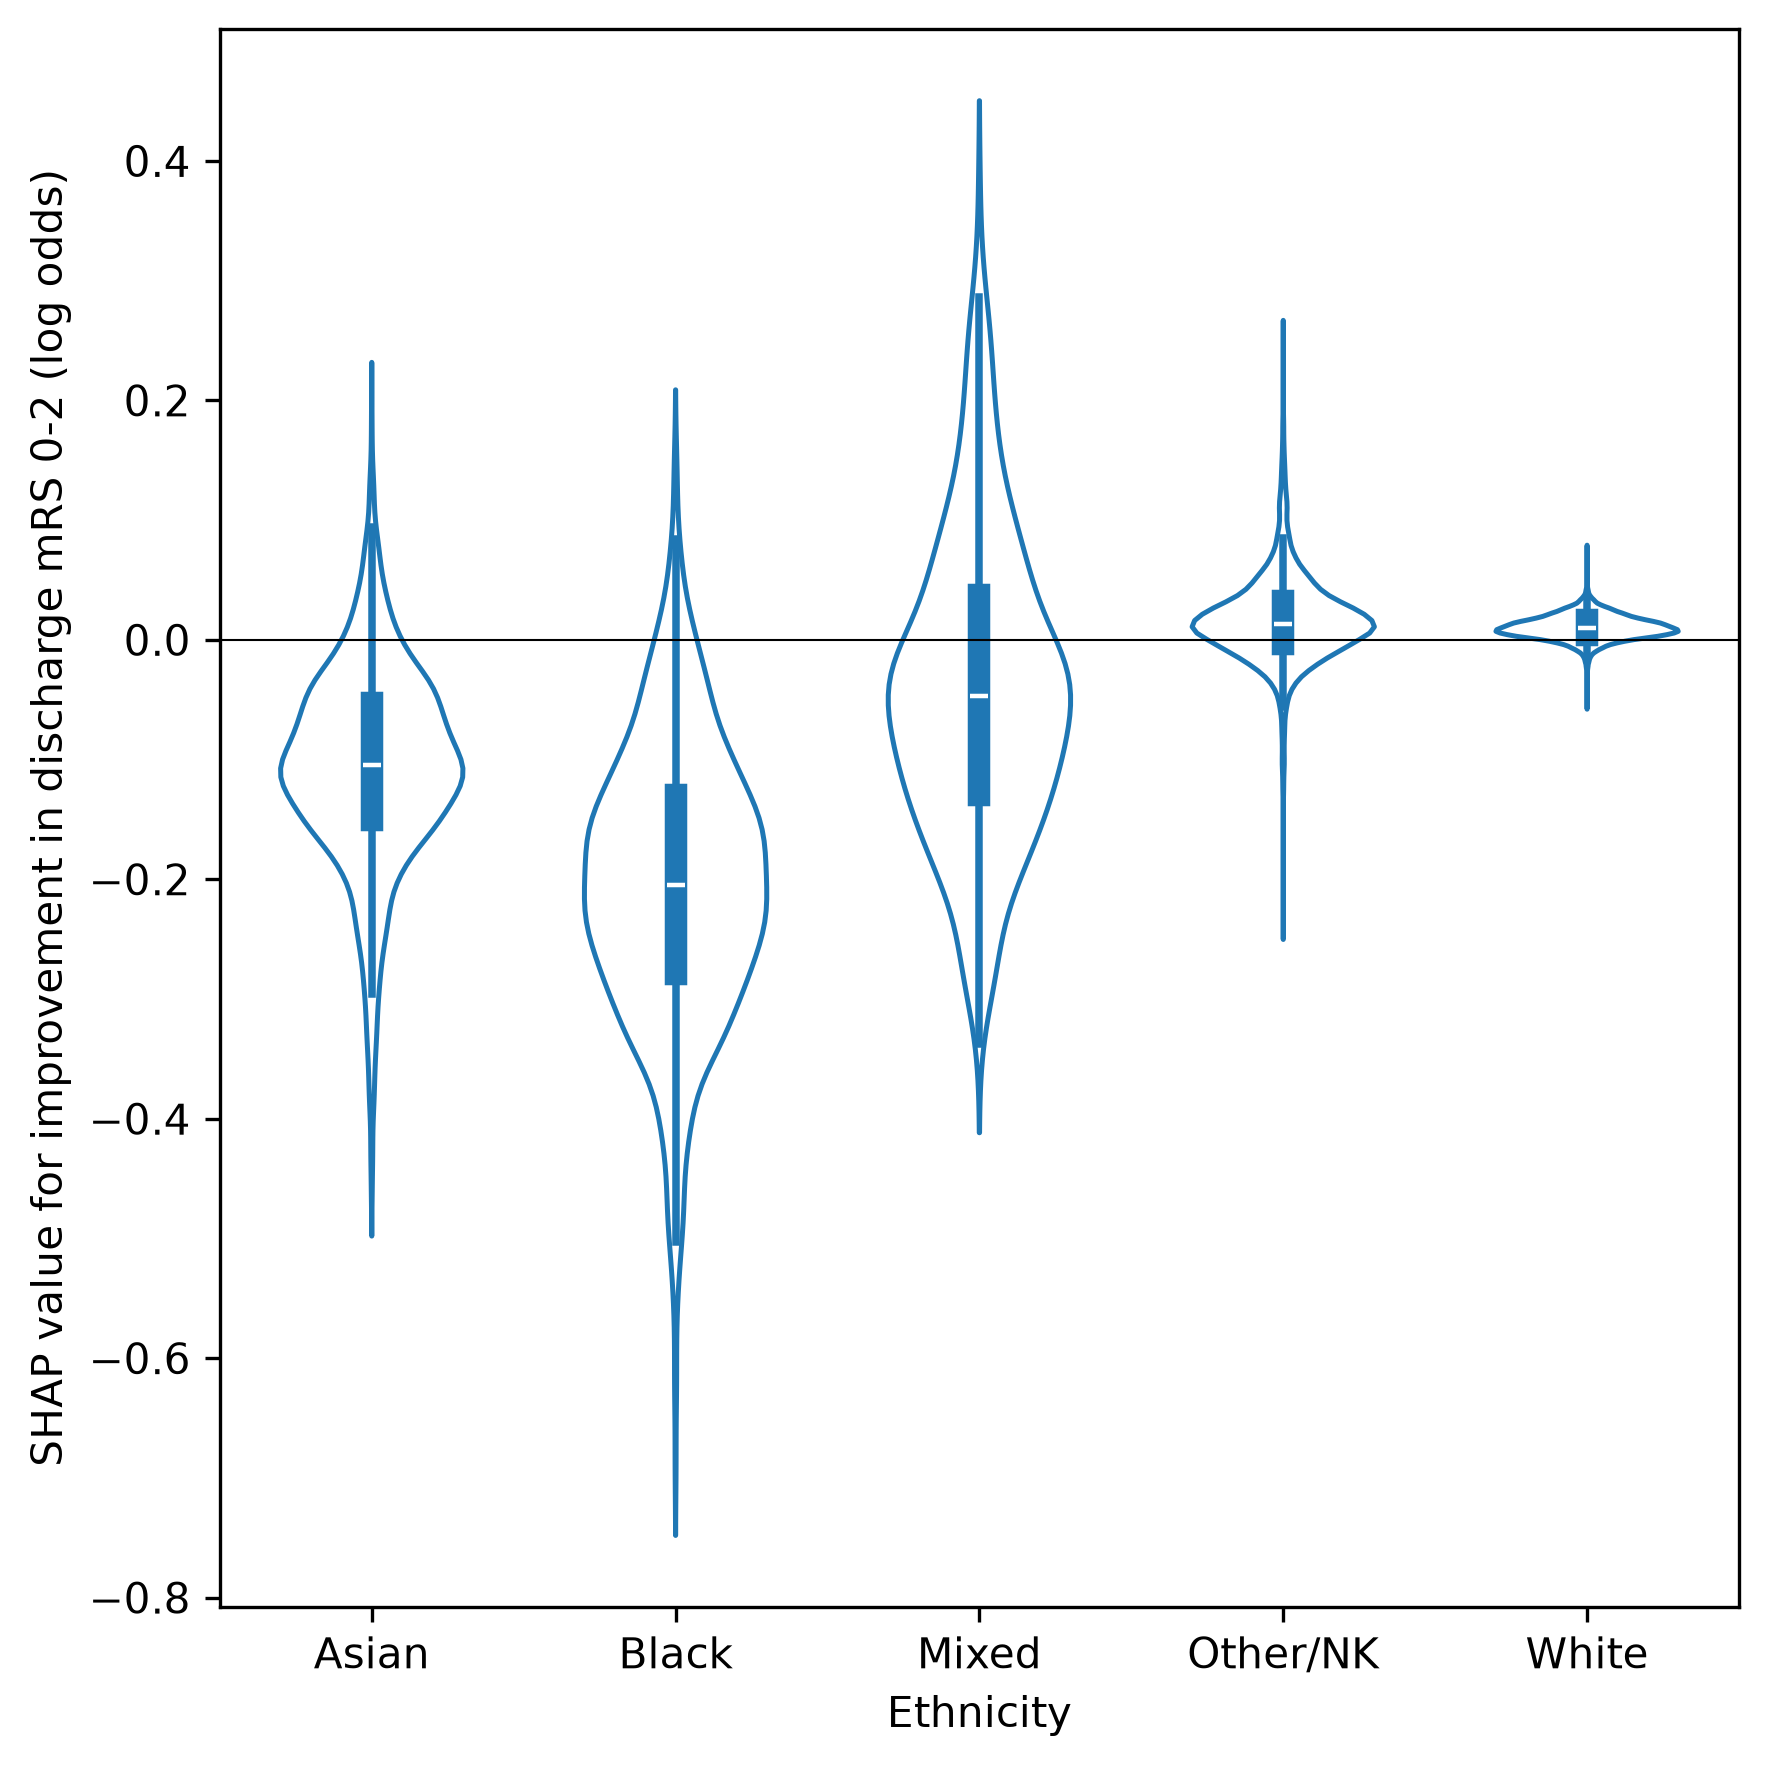
\includegraphics[width=\linewidth]{images/shap/shap_all_patients_mrs_less_than_3_ethnicity.png}
        %\caption{}
        \label{fig:bottom-left}
    \end{subfigure}
    \hfill % Adds flexible horizontal spacing
    % Bottom right image (~55% width)
    \begin{subfigure}{0.543\textwidth}
        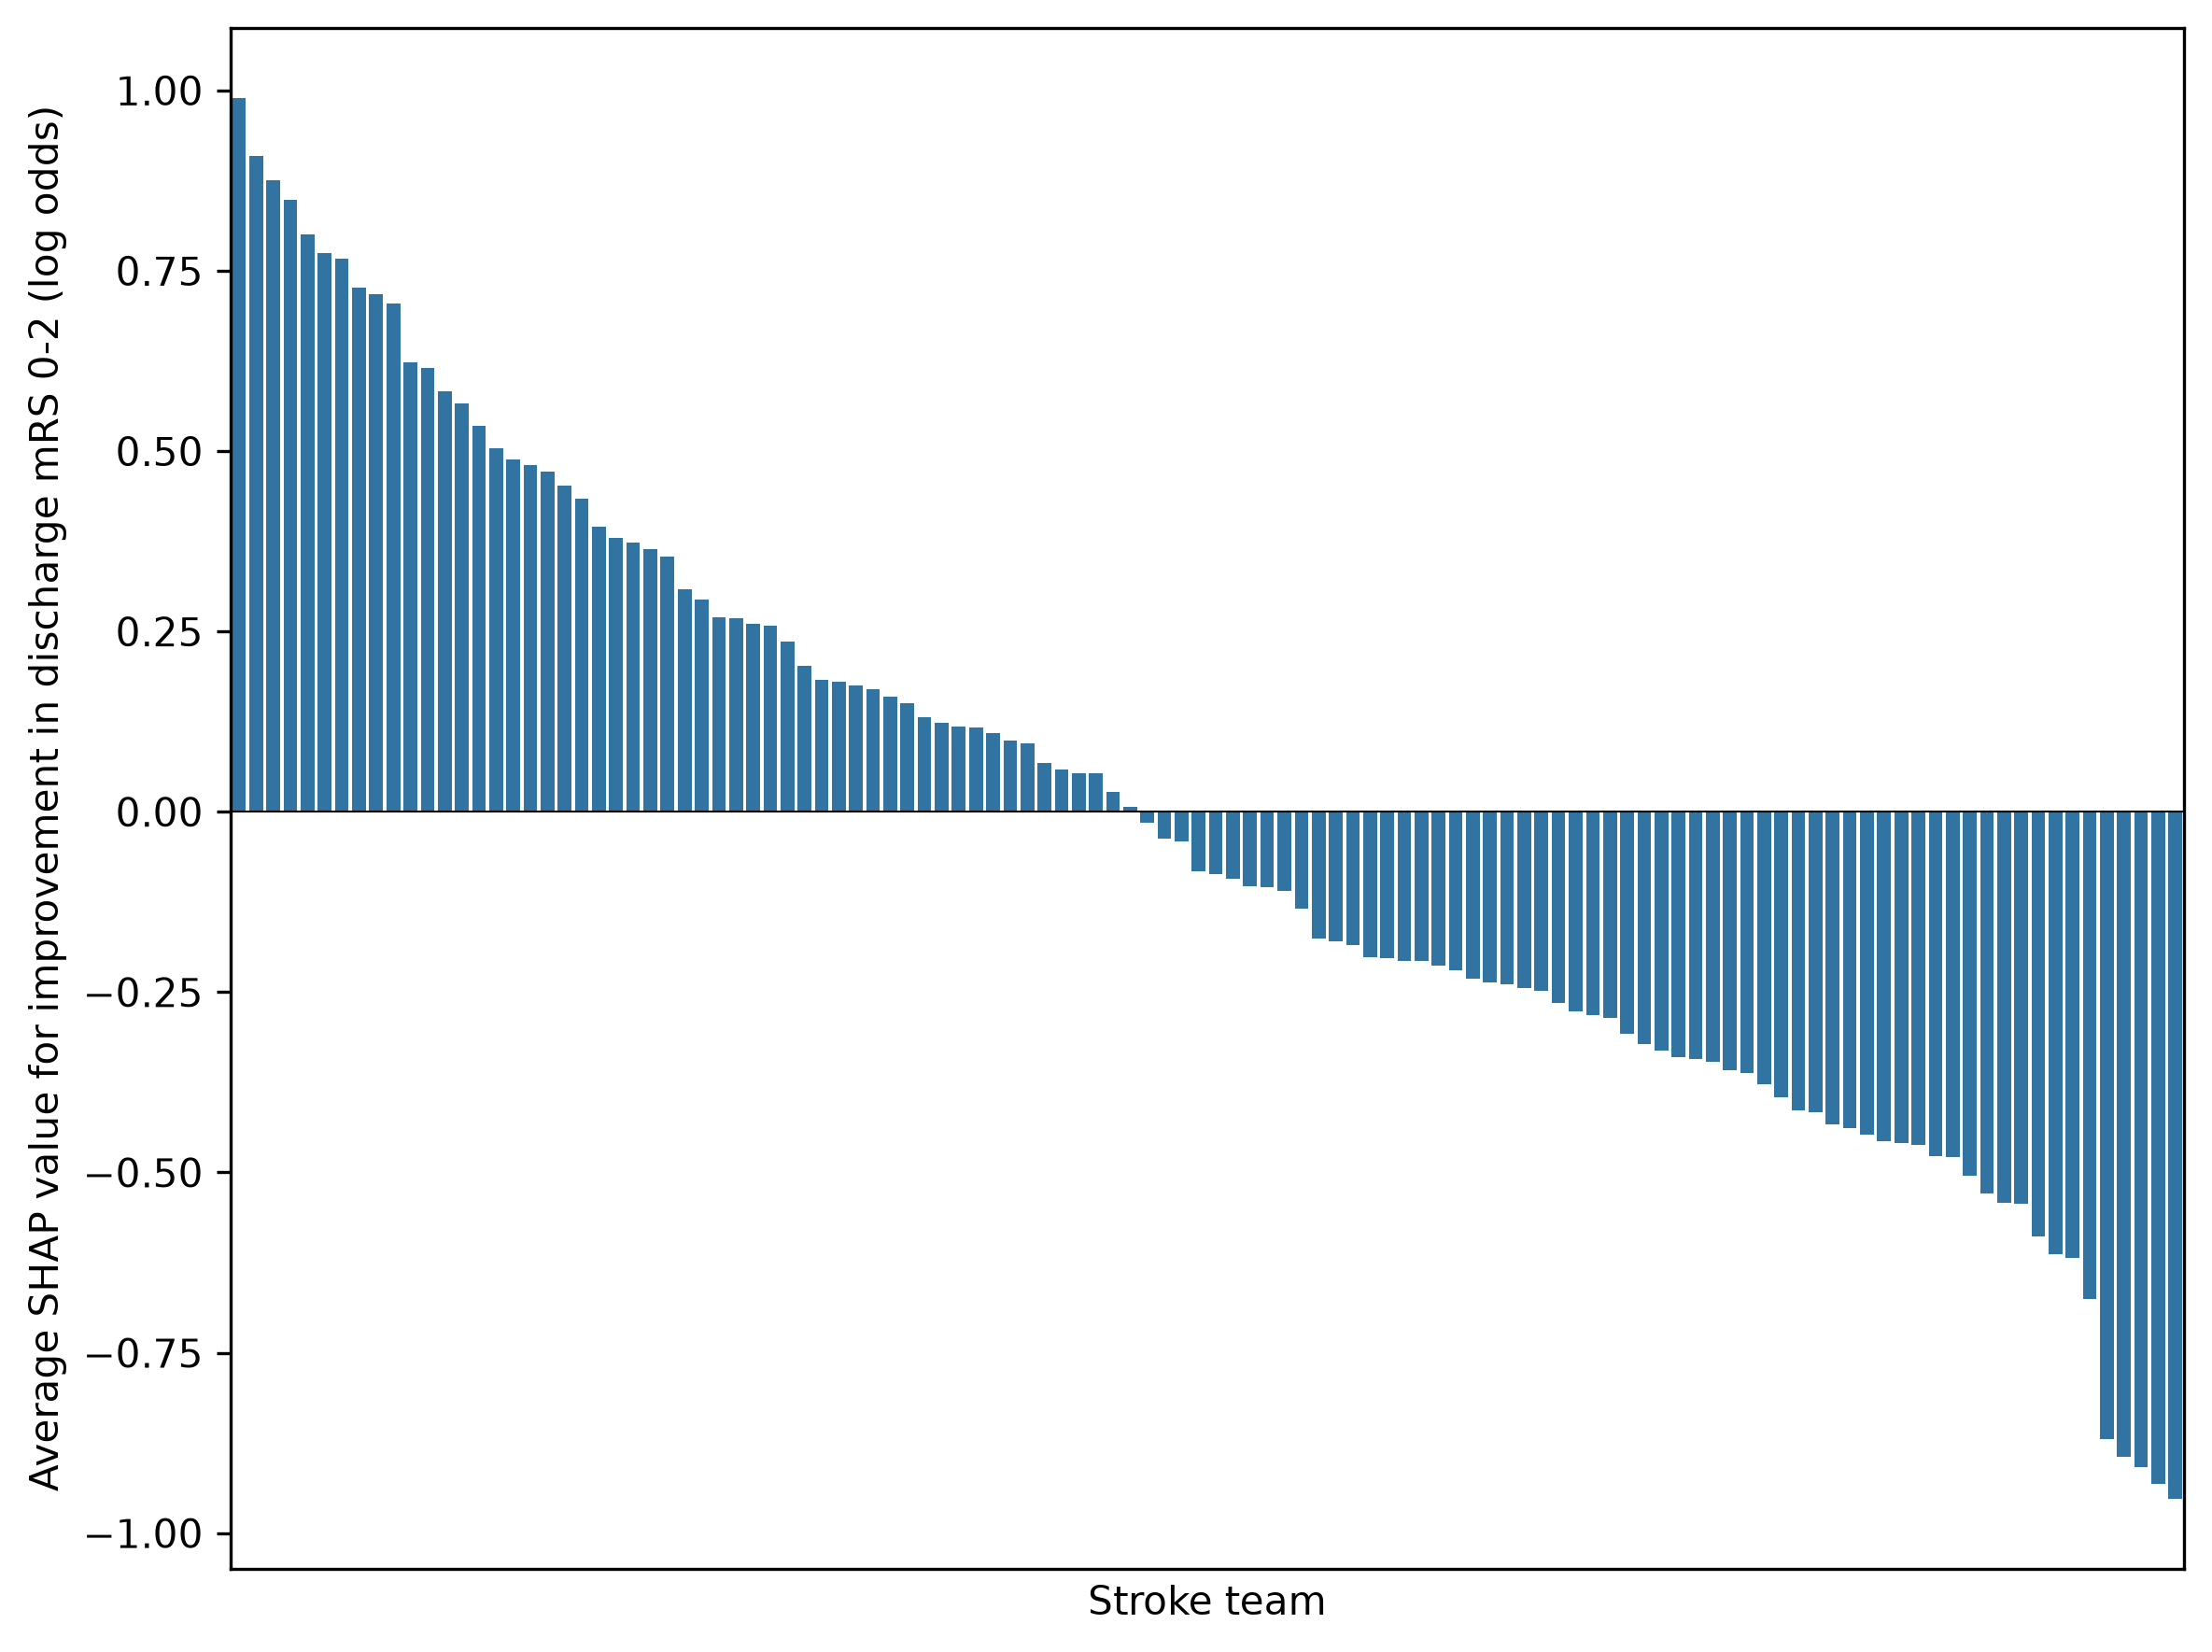
\includegraphics[width=\linewidth]{images/shap/shap_all_patients_mrs_less_than_3_stroke_team.png}
        %\caption{}
        \label{fig:bottom-right}
    \end{subfigure}

    \caption{SHAP analysis of feature contributions to predicting favourable discharge outcomes (mRS 0-2) in stroke patients. \textit{Top}: A SHAP summary plot detailing the impact of features on the model's log-odds predictions. Each point represents an individual patient instance. The position on the x-axis indicates the SHAP value, where positive values increase the predicted odds of a favourable outcome, and negative values decrease it. For continuous and binary variables, colour represents the original feature value (red indicating high values; blue indicating low values). Categorical variables (\textit{stroke team} and \textit{ethnicity}) are plotted in grey. \textit{Bottom left}: Violin plots illustrating the distribution of SHAP values across distinct ethnic groups. This panel highlights the marginal impact and variance of ethnicity on the model’s prediction for disability outcome. \textit{Bottom Right}: A ranked bar chart displaying the average SHAP value associated with each individual stroke team. This panel visualizes institutional variation, reflecting the contribution of the treating stroke team to the predicted patient outcome after accounting for patient-level clinical characteristics.}
    \label{fig:shap_mrs0-2_no_all}
\end{figure}

%% Untreated patients

\begin{figure}[htbp]
    \centering
    
    % Top image (Full width)
    \begin{subfigure}{0.50\textwidth}
        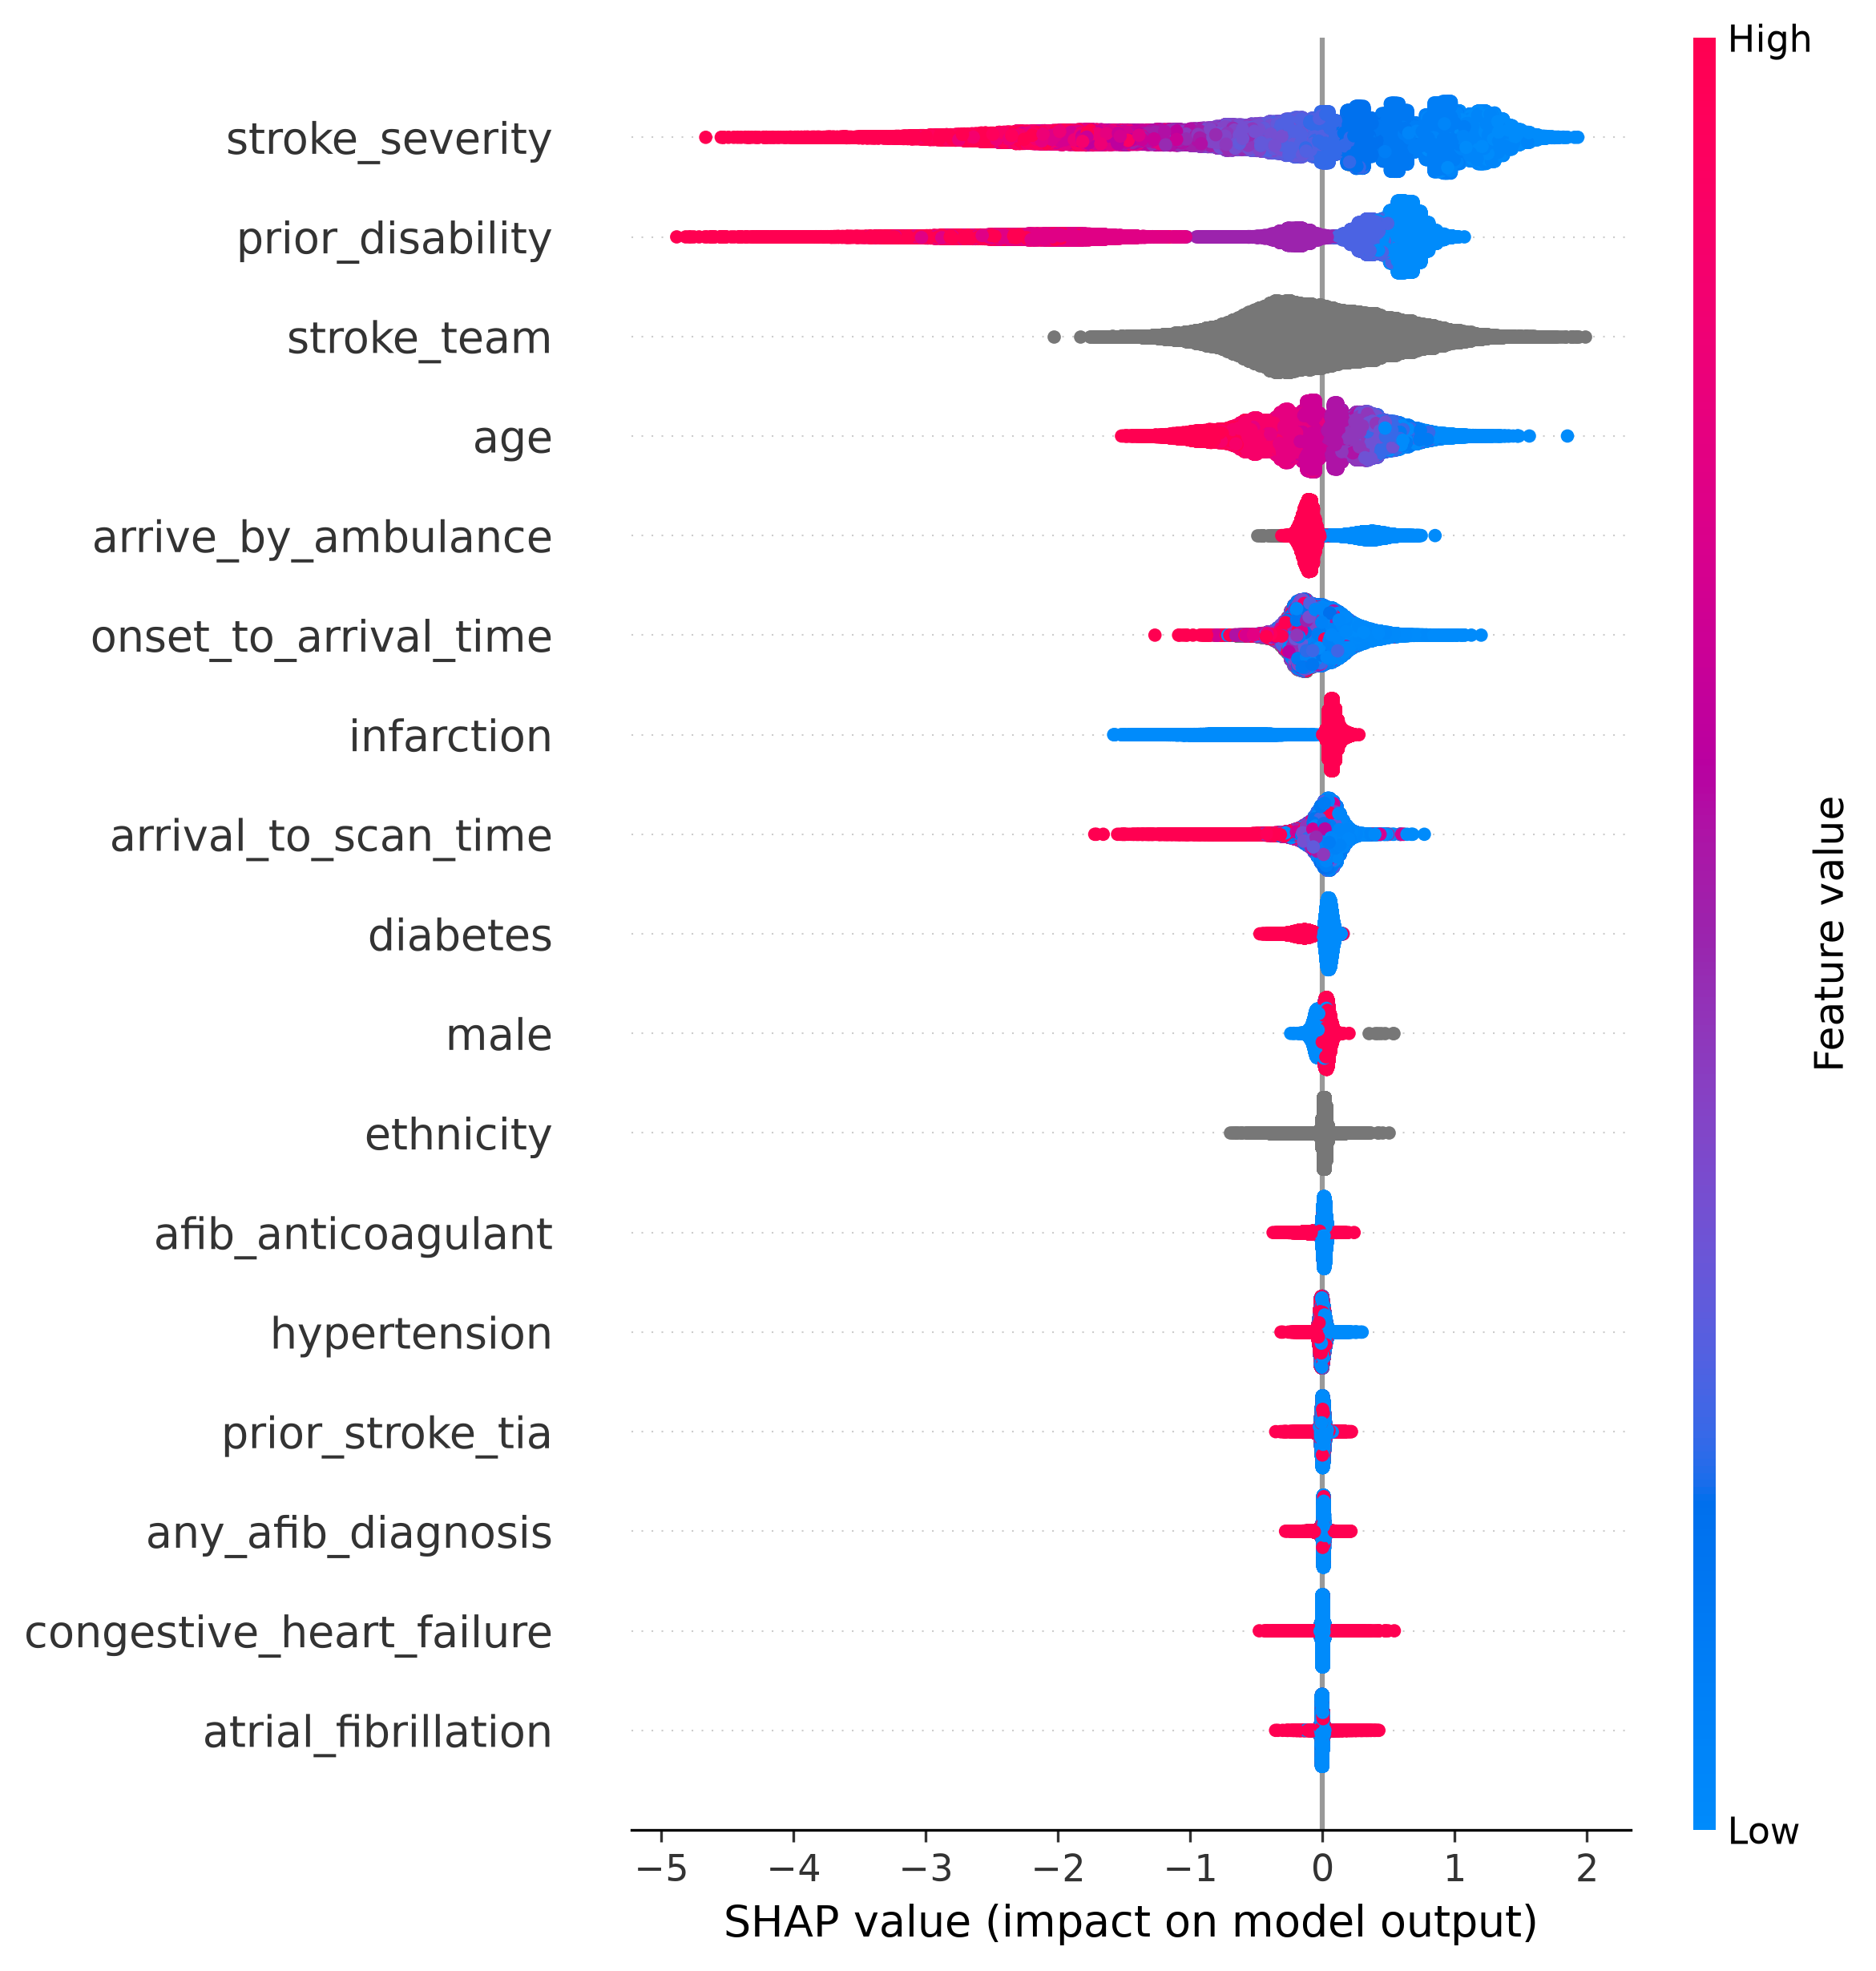
\includegraphics[width=\linewidth]{images/shap/shap_untreated_patients_mrs_less_than_3.png}
        %\caption{}
        \label{fig:top}
    \end{subfigure}

    \vspace{0.5cm} % Optional vertical space between rows

    % Bottom left image (~45% width)
    \begin{subfigure}{0.407\textwidth}
        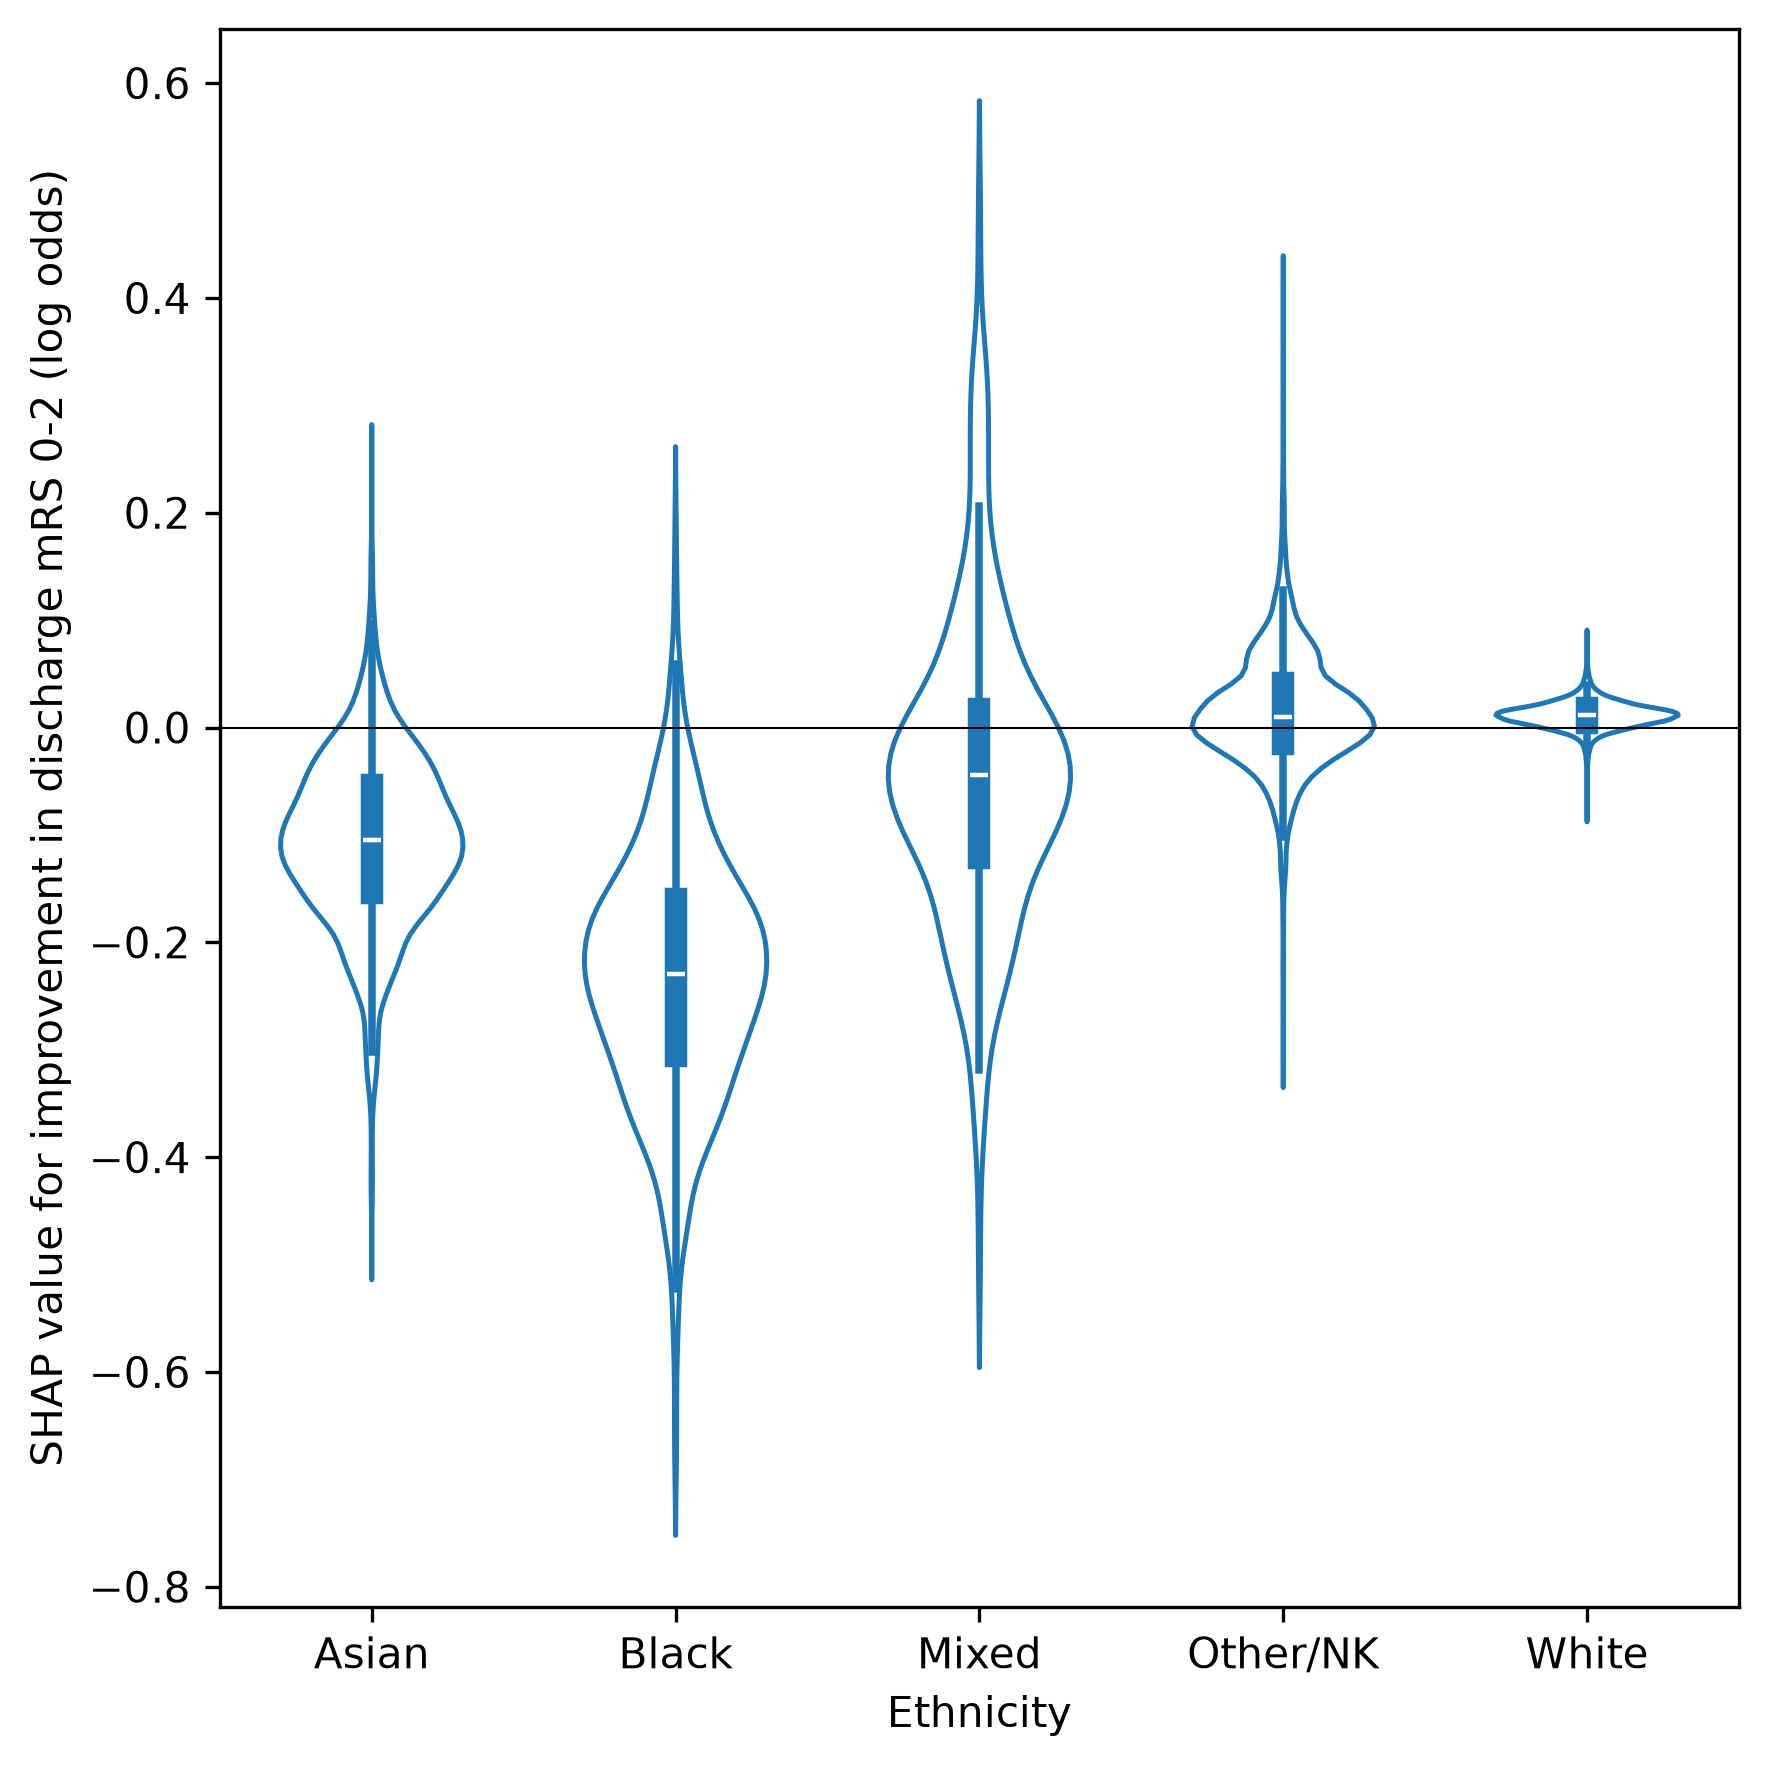
\includegraphics[width=\linewidth]{images/shap/shap_untreated_patients_mrs_less_than_3_ethnicity.png}
        %\caption{}
        \label{fig:bottom-left}
    \end{subfigure}
    \hfill % Adds flexible horizontal spacing
    % Bottom right image (~55% width)
    \begin{subfigure}{0.543\textwidth}
        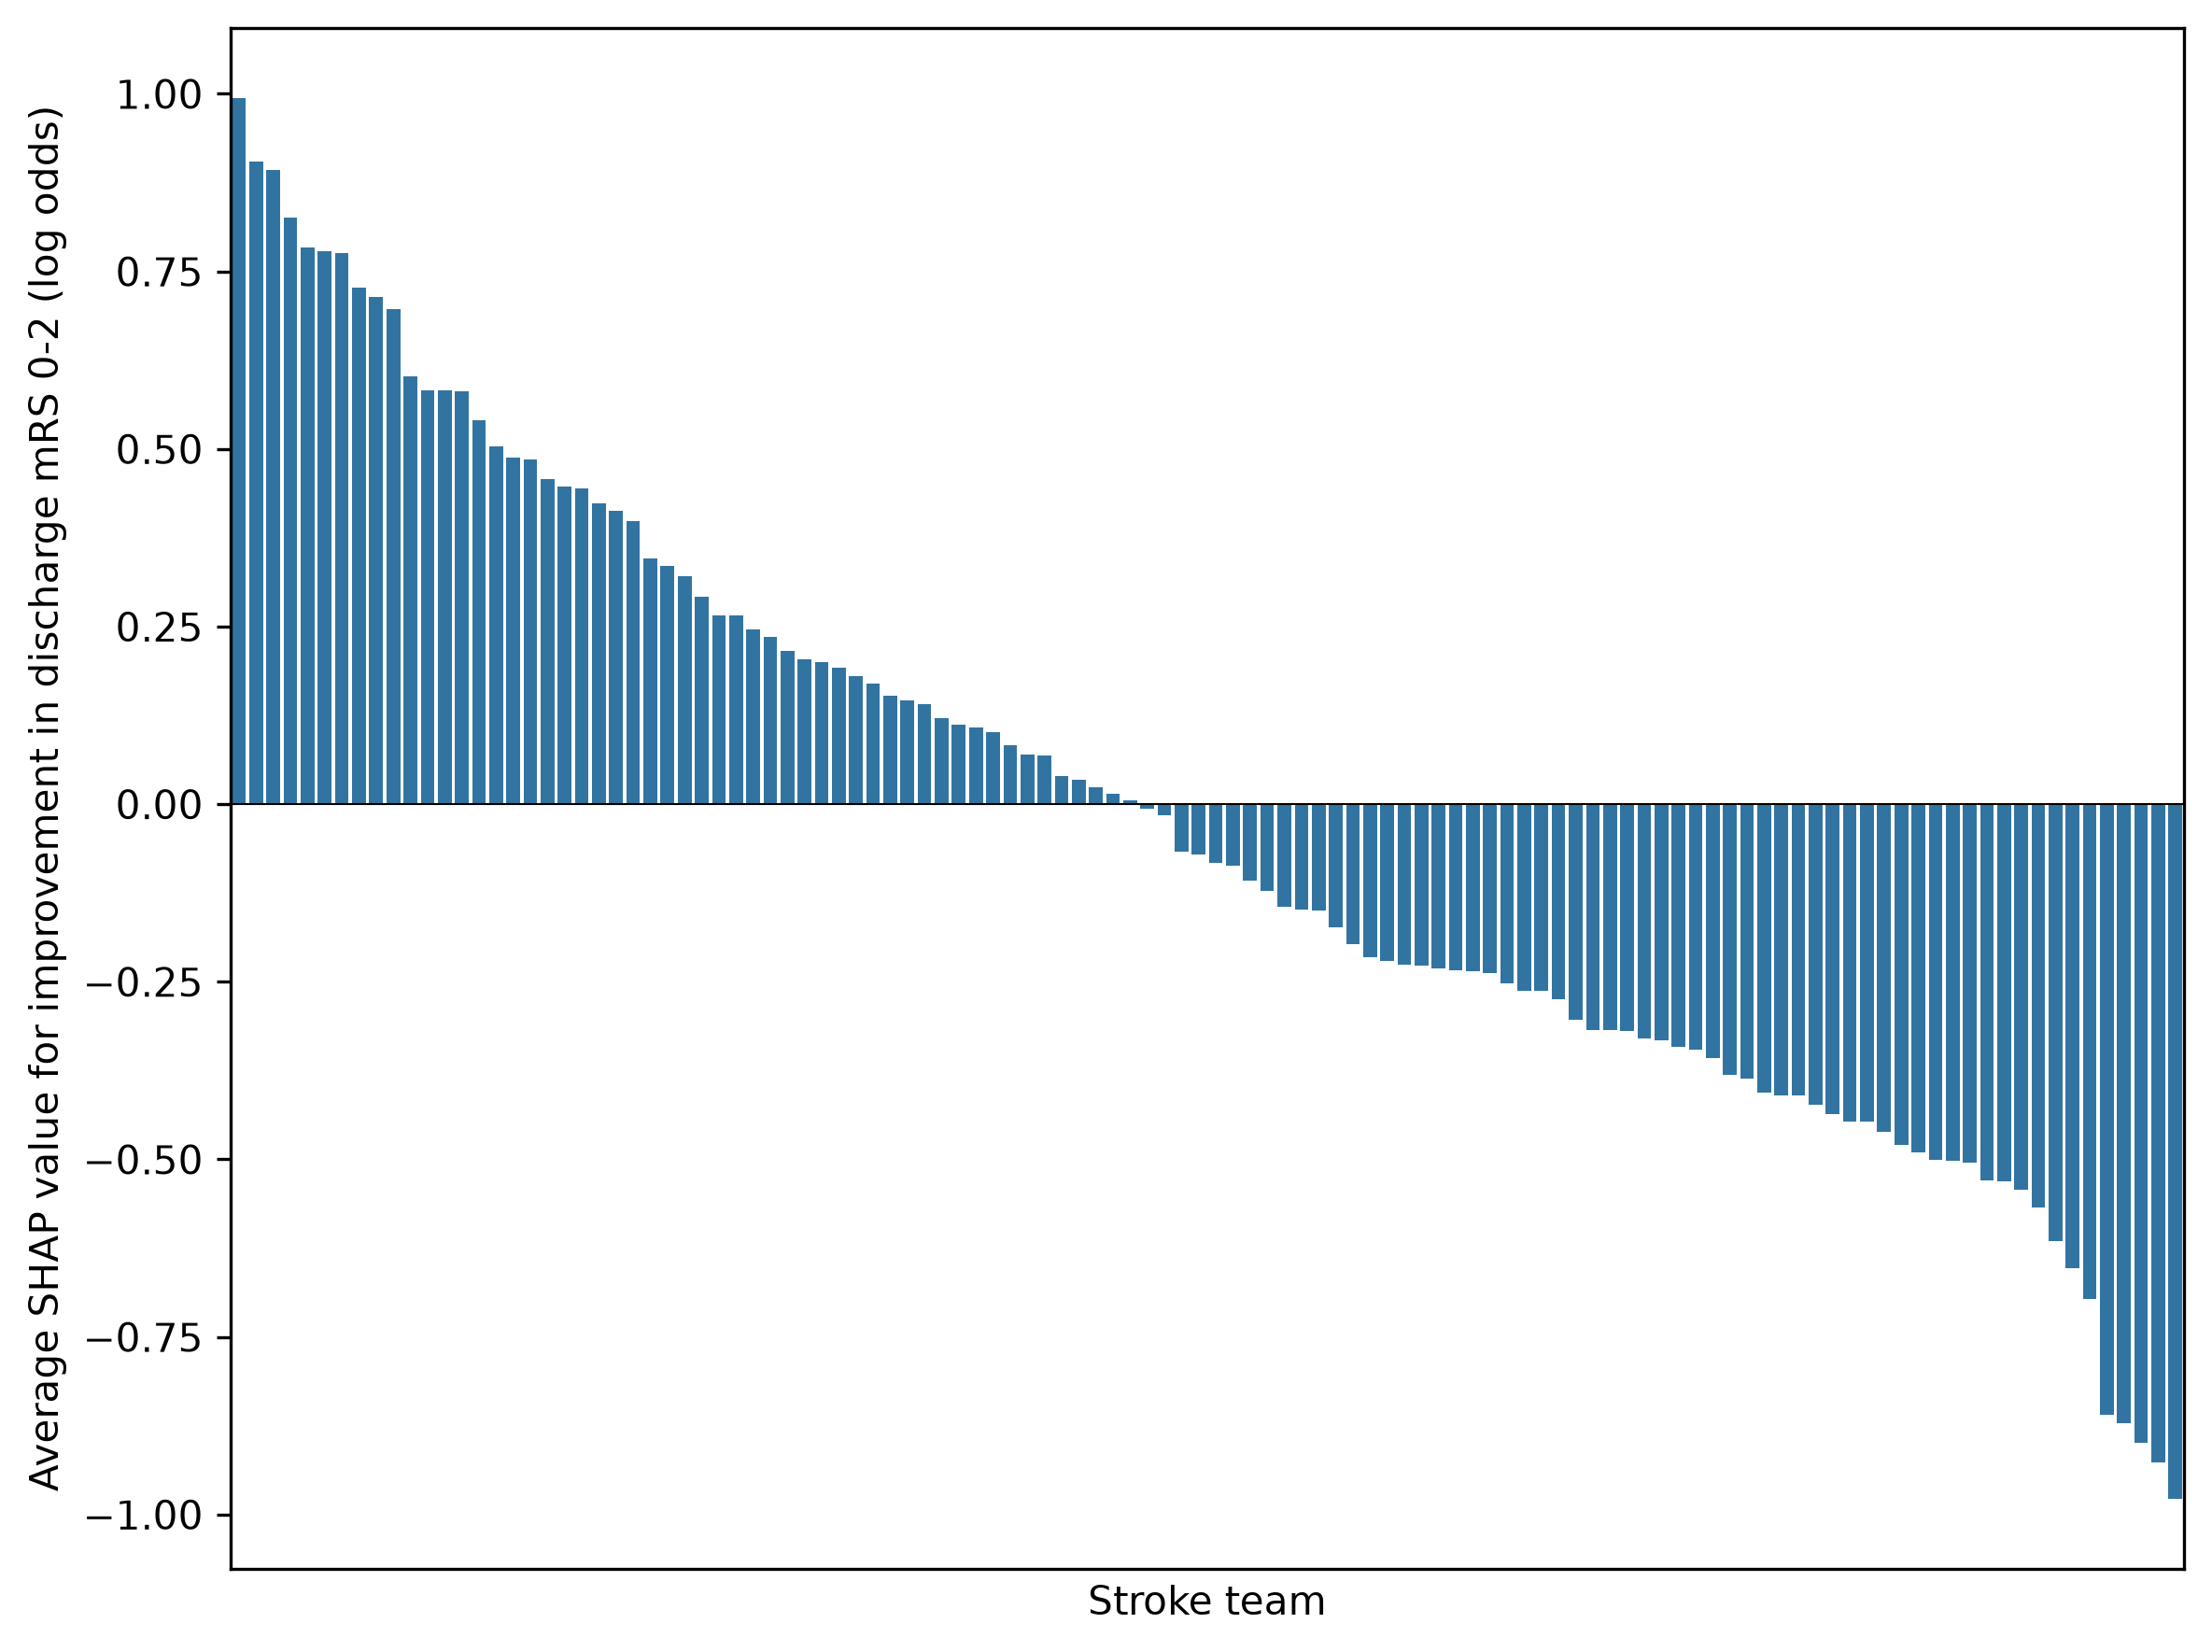
\includegraphics[width=\linewidth]{images/shap/shap_untreated_patients_mrs_less_than_3_stroke_team.png}
        %\caption{}
        \label{fig:bottom-right}
    \end{subfigure}

    \caption{SHAP analysis of feature contributions to predicting favourable discharge outcomes (mRS 0-2) in stroke patients who did not receive thrombolysis or thrombectomy. \textit{Top}: A SHAP summary plot detailing the impact of features on the model's log-odds predictions. Each point represents an individual patient instance. The position on the x-axis indicates the SHAP value, where positive values increase the predicted odds of a favourable outcome, and negative values decrease it. For continuous and binary variables, colour represents the original feature value (red indicating high values; blue indicating low values). Categorical variables (\textit{stroke team} and \textit{ethnicity}) are plotted in grey. \textit{Bottom left}: Violin plots illustrating the distribution of SHAP values across distinct ethnic groups. This panel highlights the marginal impact and variance of ethnicity on the model’s prediction for disability outcome. \textit{Bottom Right}: A ranked bar chart displaying the average SHAP value associated with each individual stroke team. This panel visualizes institutional variation, reflecting the contribution of the treating stroke team to the predicted patient outcome after accounting for patient-level clinical characteristics.}
    \label{fig:shap_mrs0-2_no_treatment}
\end{figure}

%%%%%%%%%%% Survival %%%%%%%%%%%%%%%

%% All patients

\begin{figure}[htbp]
    \centering
    
    % Top image (Full width)
    \begin{subfigure}{0.50\textwidth}
        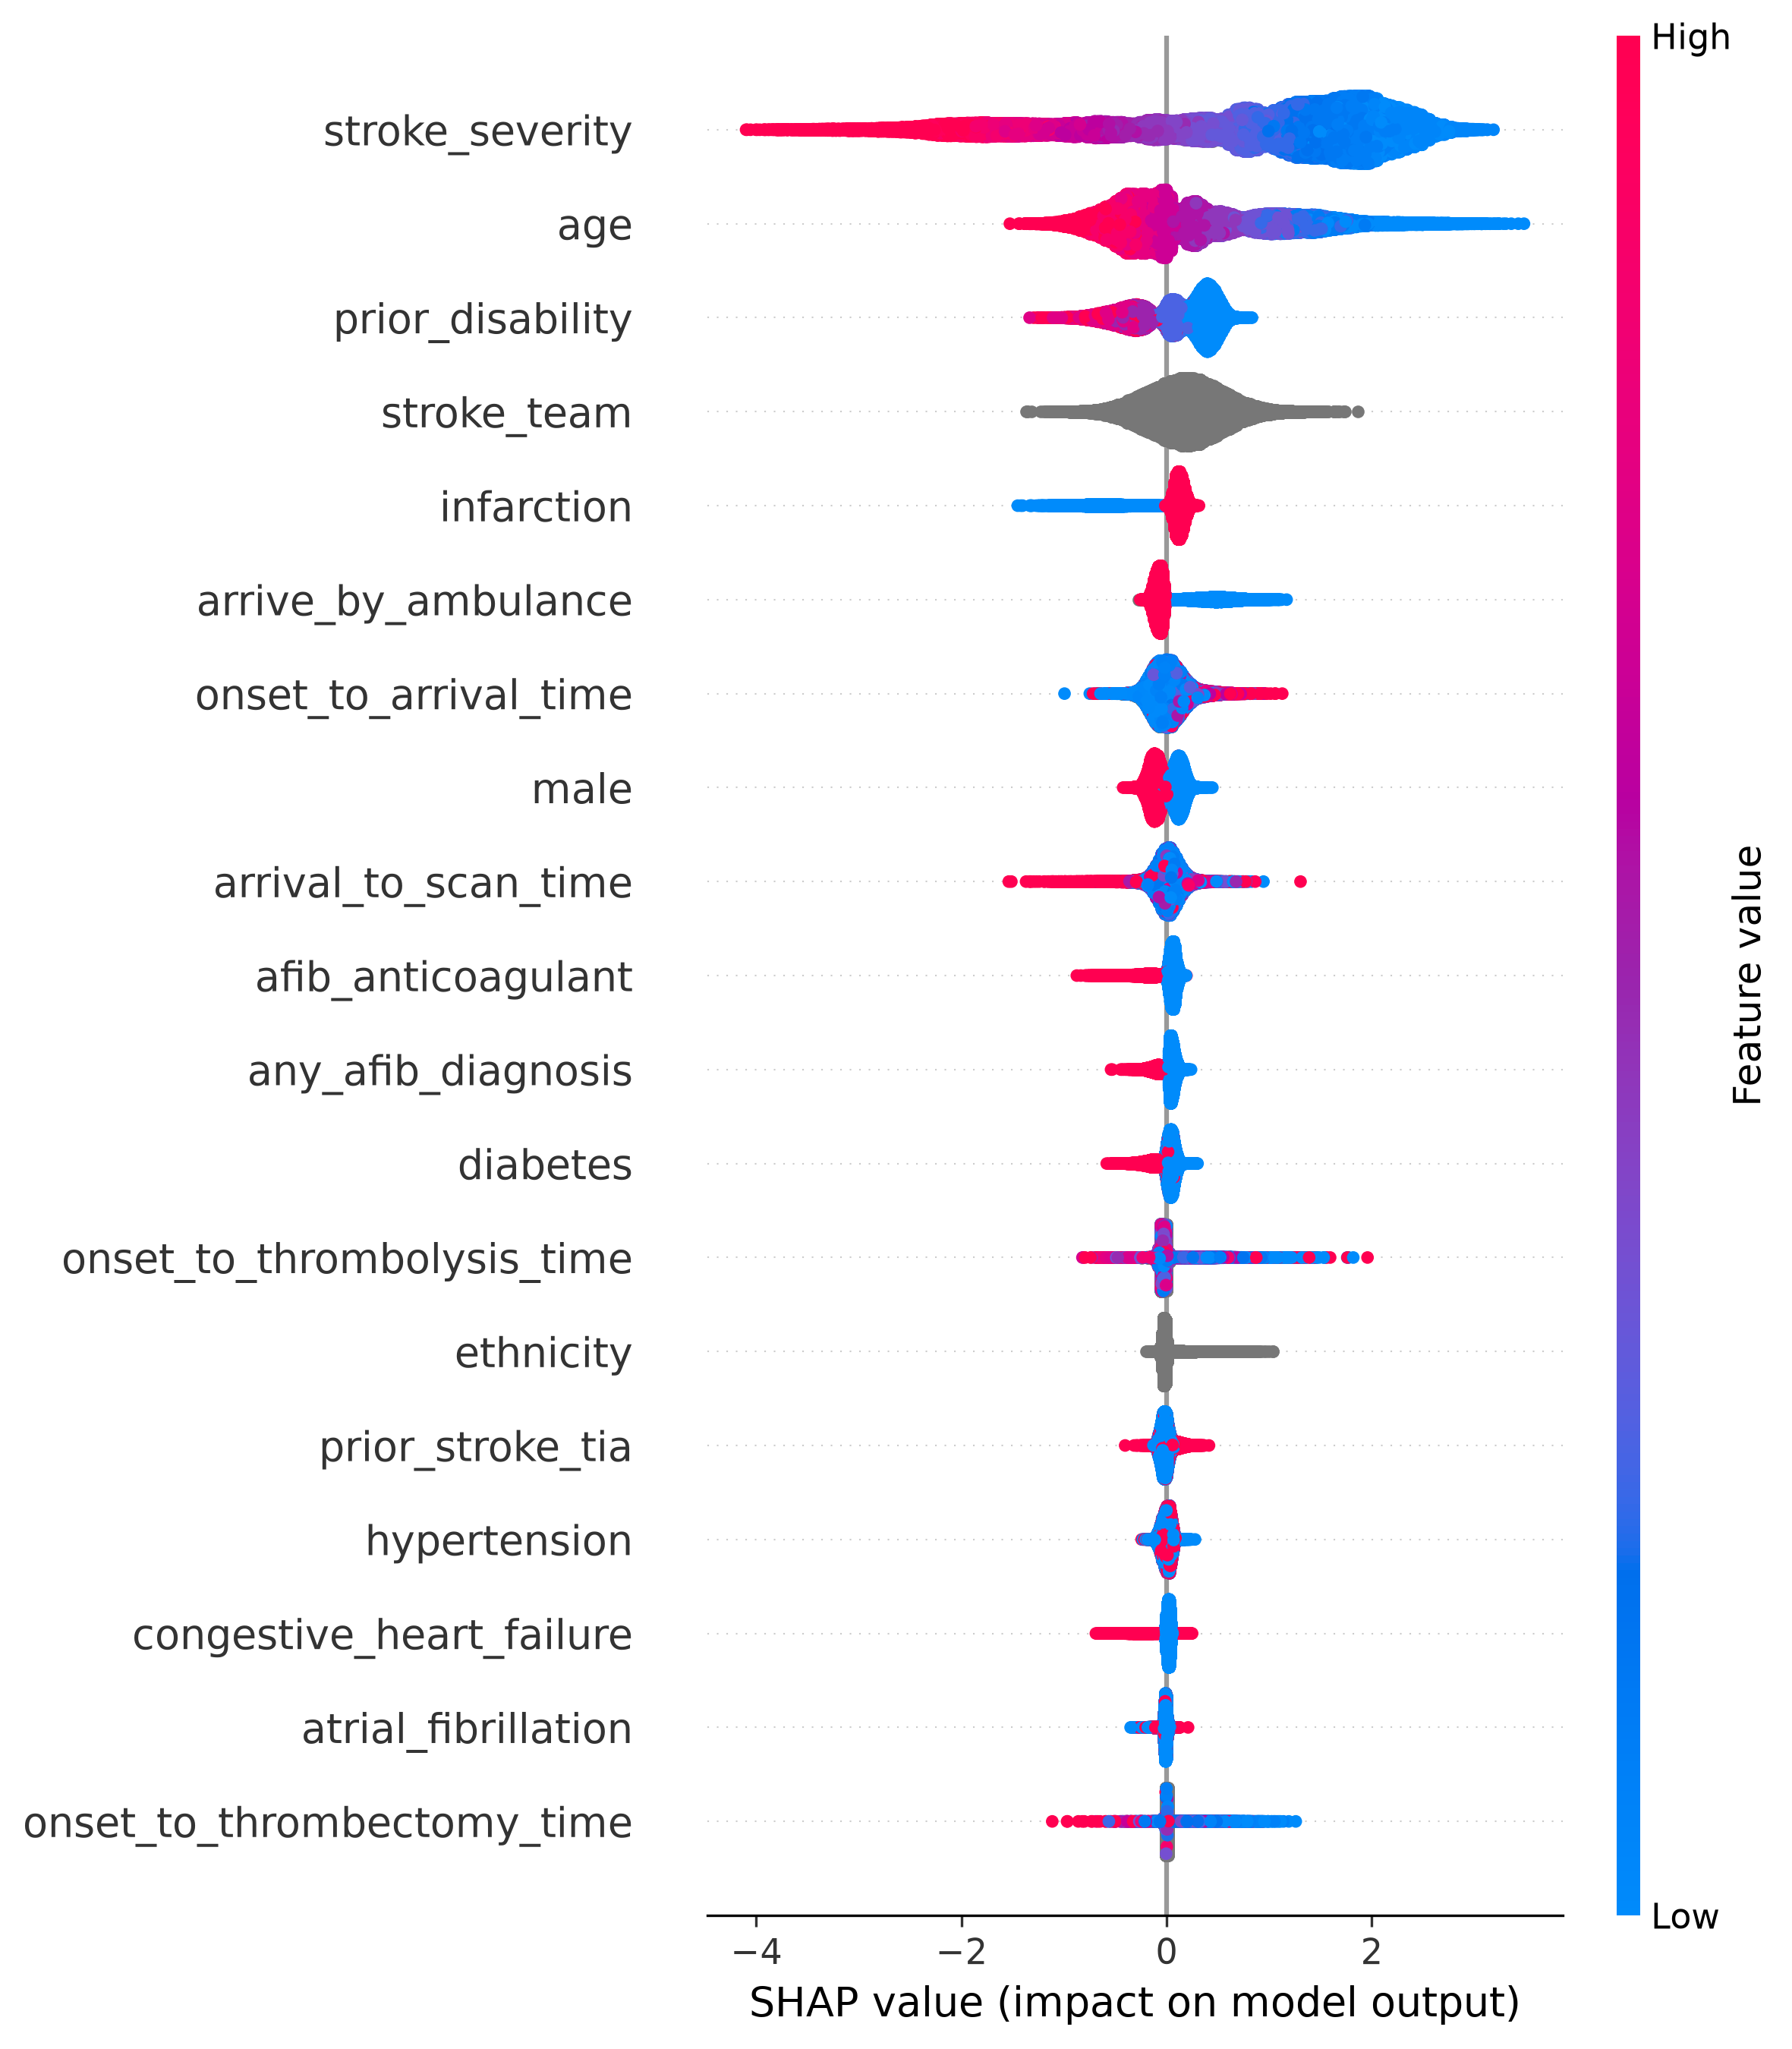
\includegraphics[width=\linewidth]{images/shap/shap_all_patients_survival.png}
        %\caption{}
        \label{fig:top}
    \end{subfigure}

    \vspace{0.5cm} % Optional vertical space between rows

    % Bottom left image (~45% width)
    \begin{subfigure}{0.407\textwidth}
        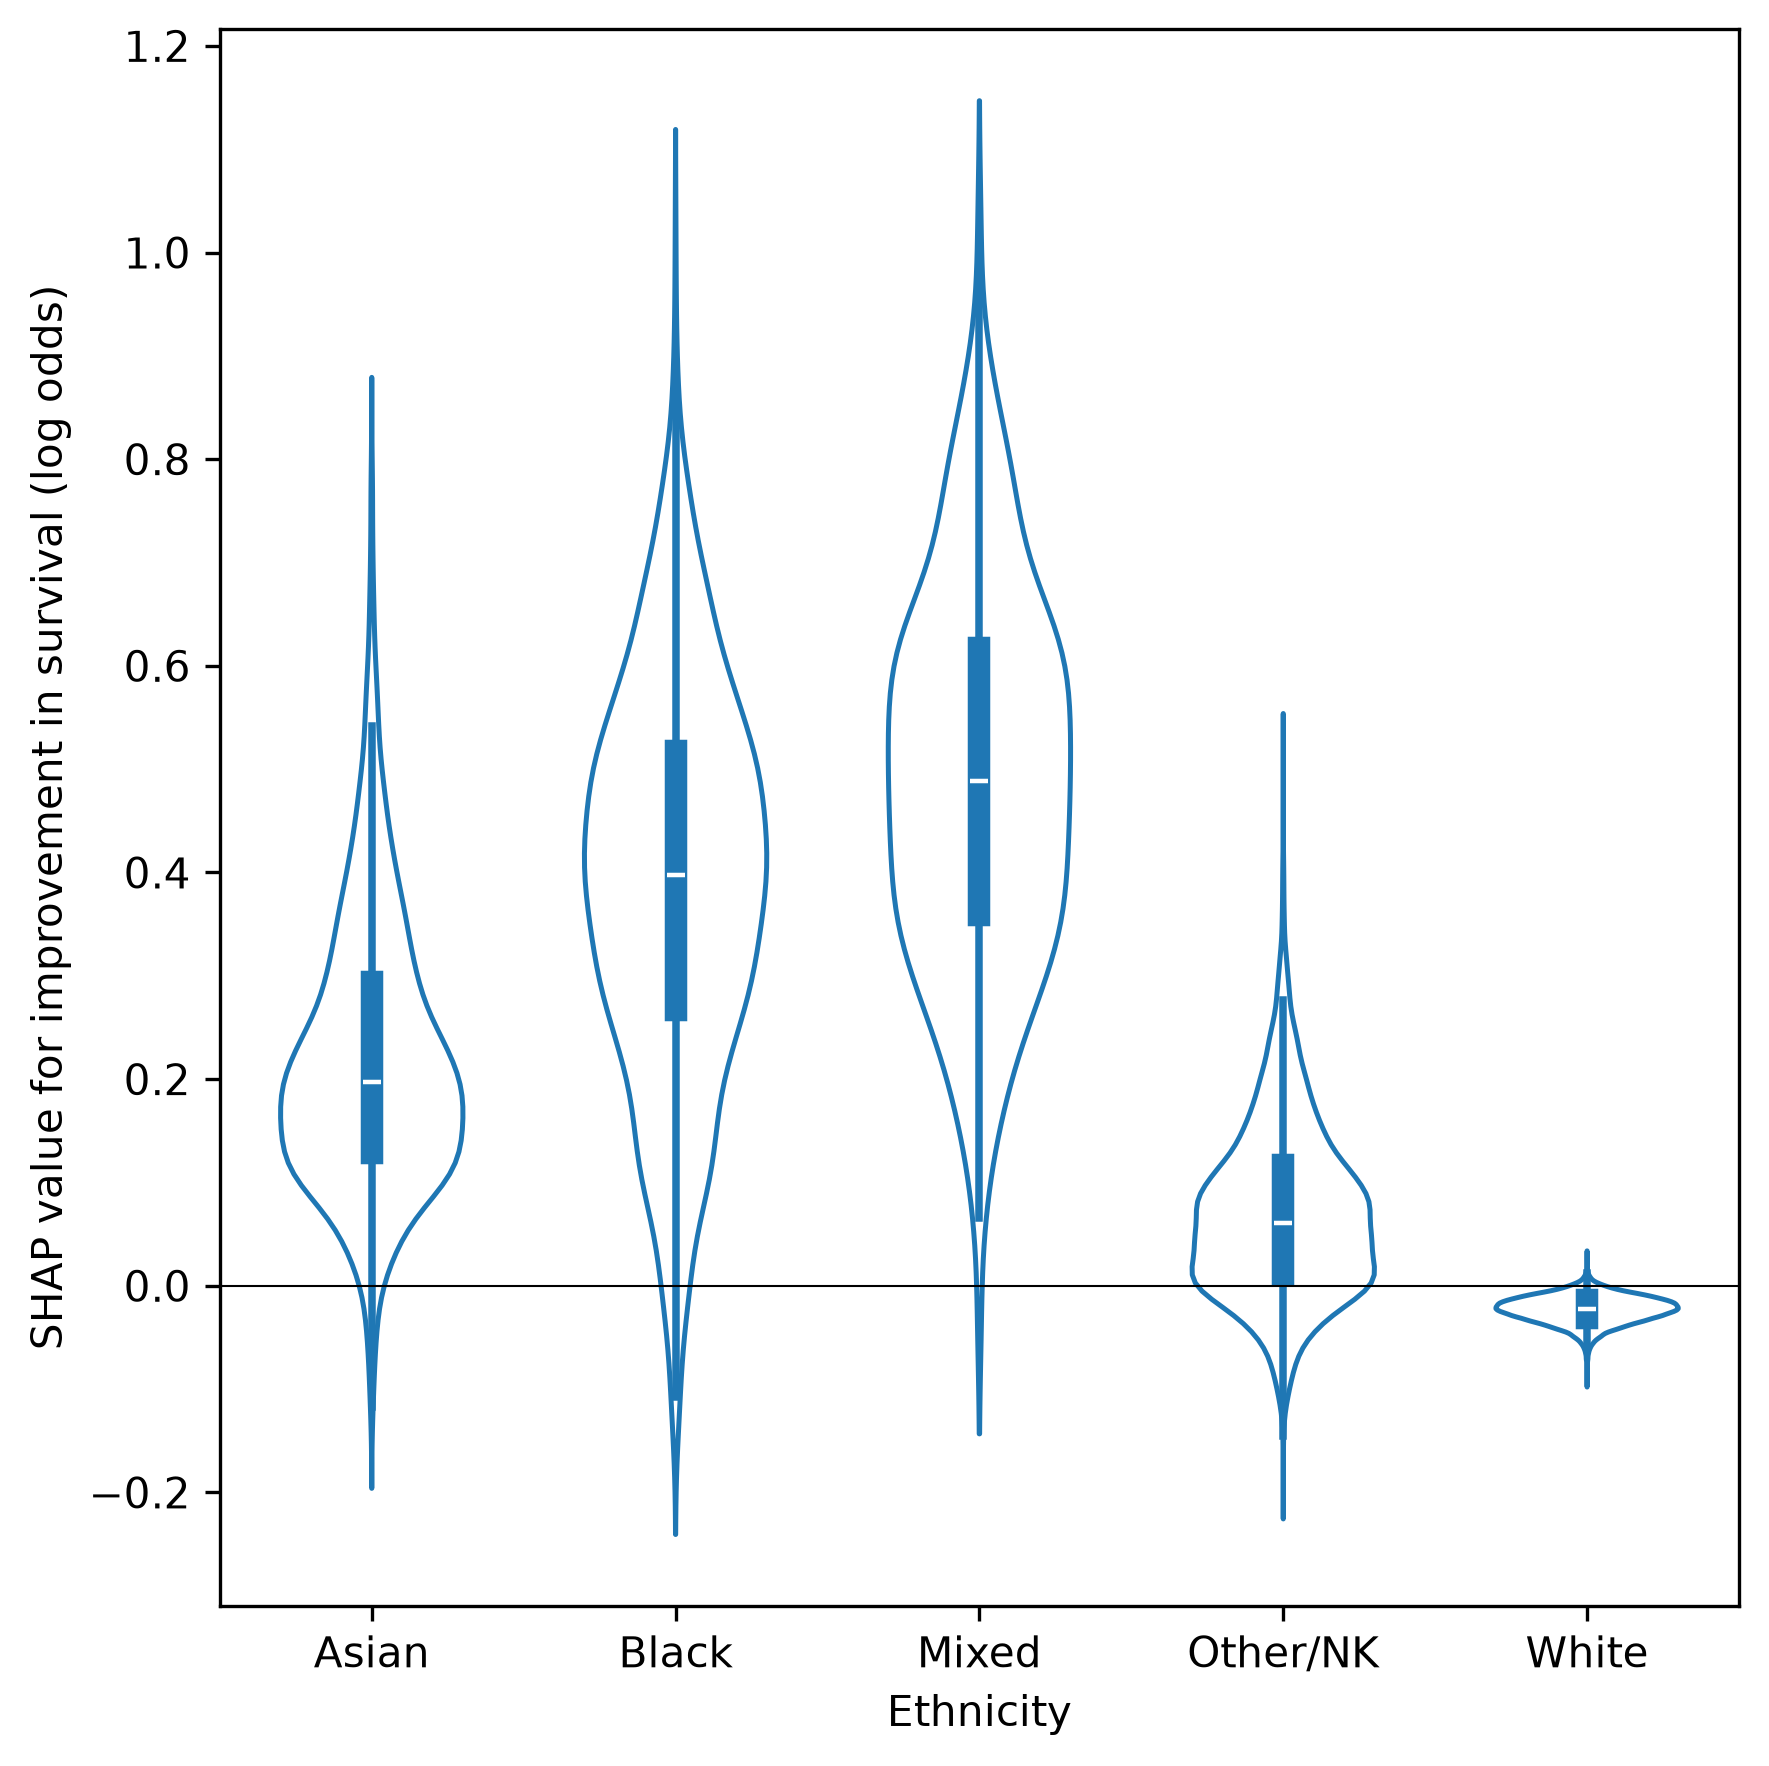
\includegraphics[width=\linewidth]{images/shap/shap_all_patients_survival_ethnicity.png}
        %\caption{}
        \label{fig:bottom-left}
    \end{subfigure}
    \hfill % Adds flexible horizontal spacing
    % Bottom right image (~55% width)
    \begin{subfigure}{0.543\textwidth}
        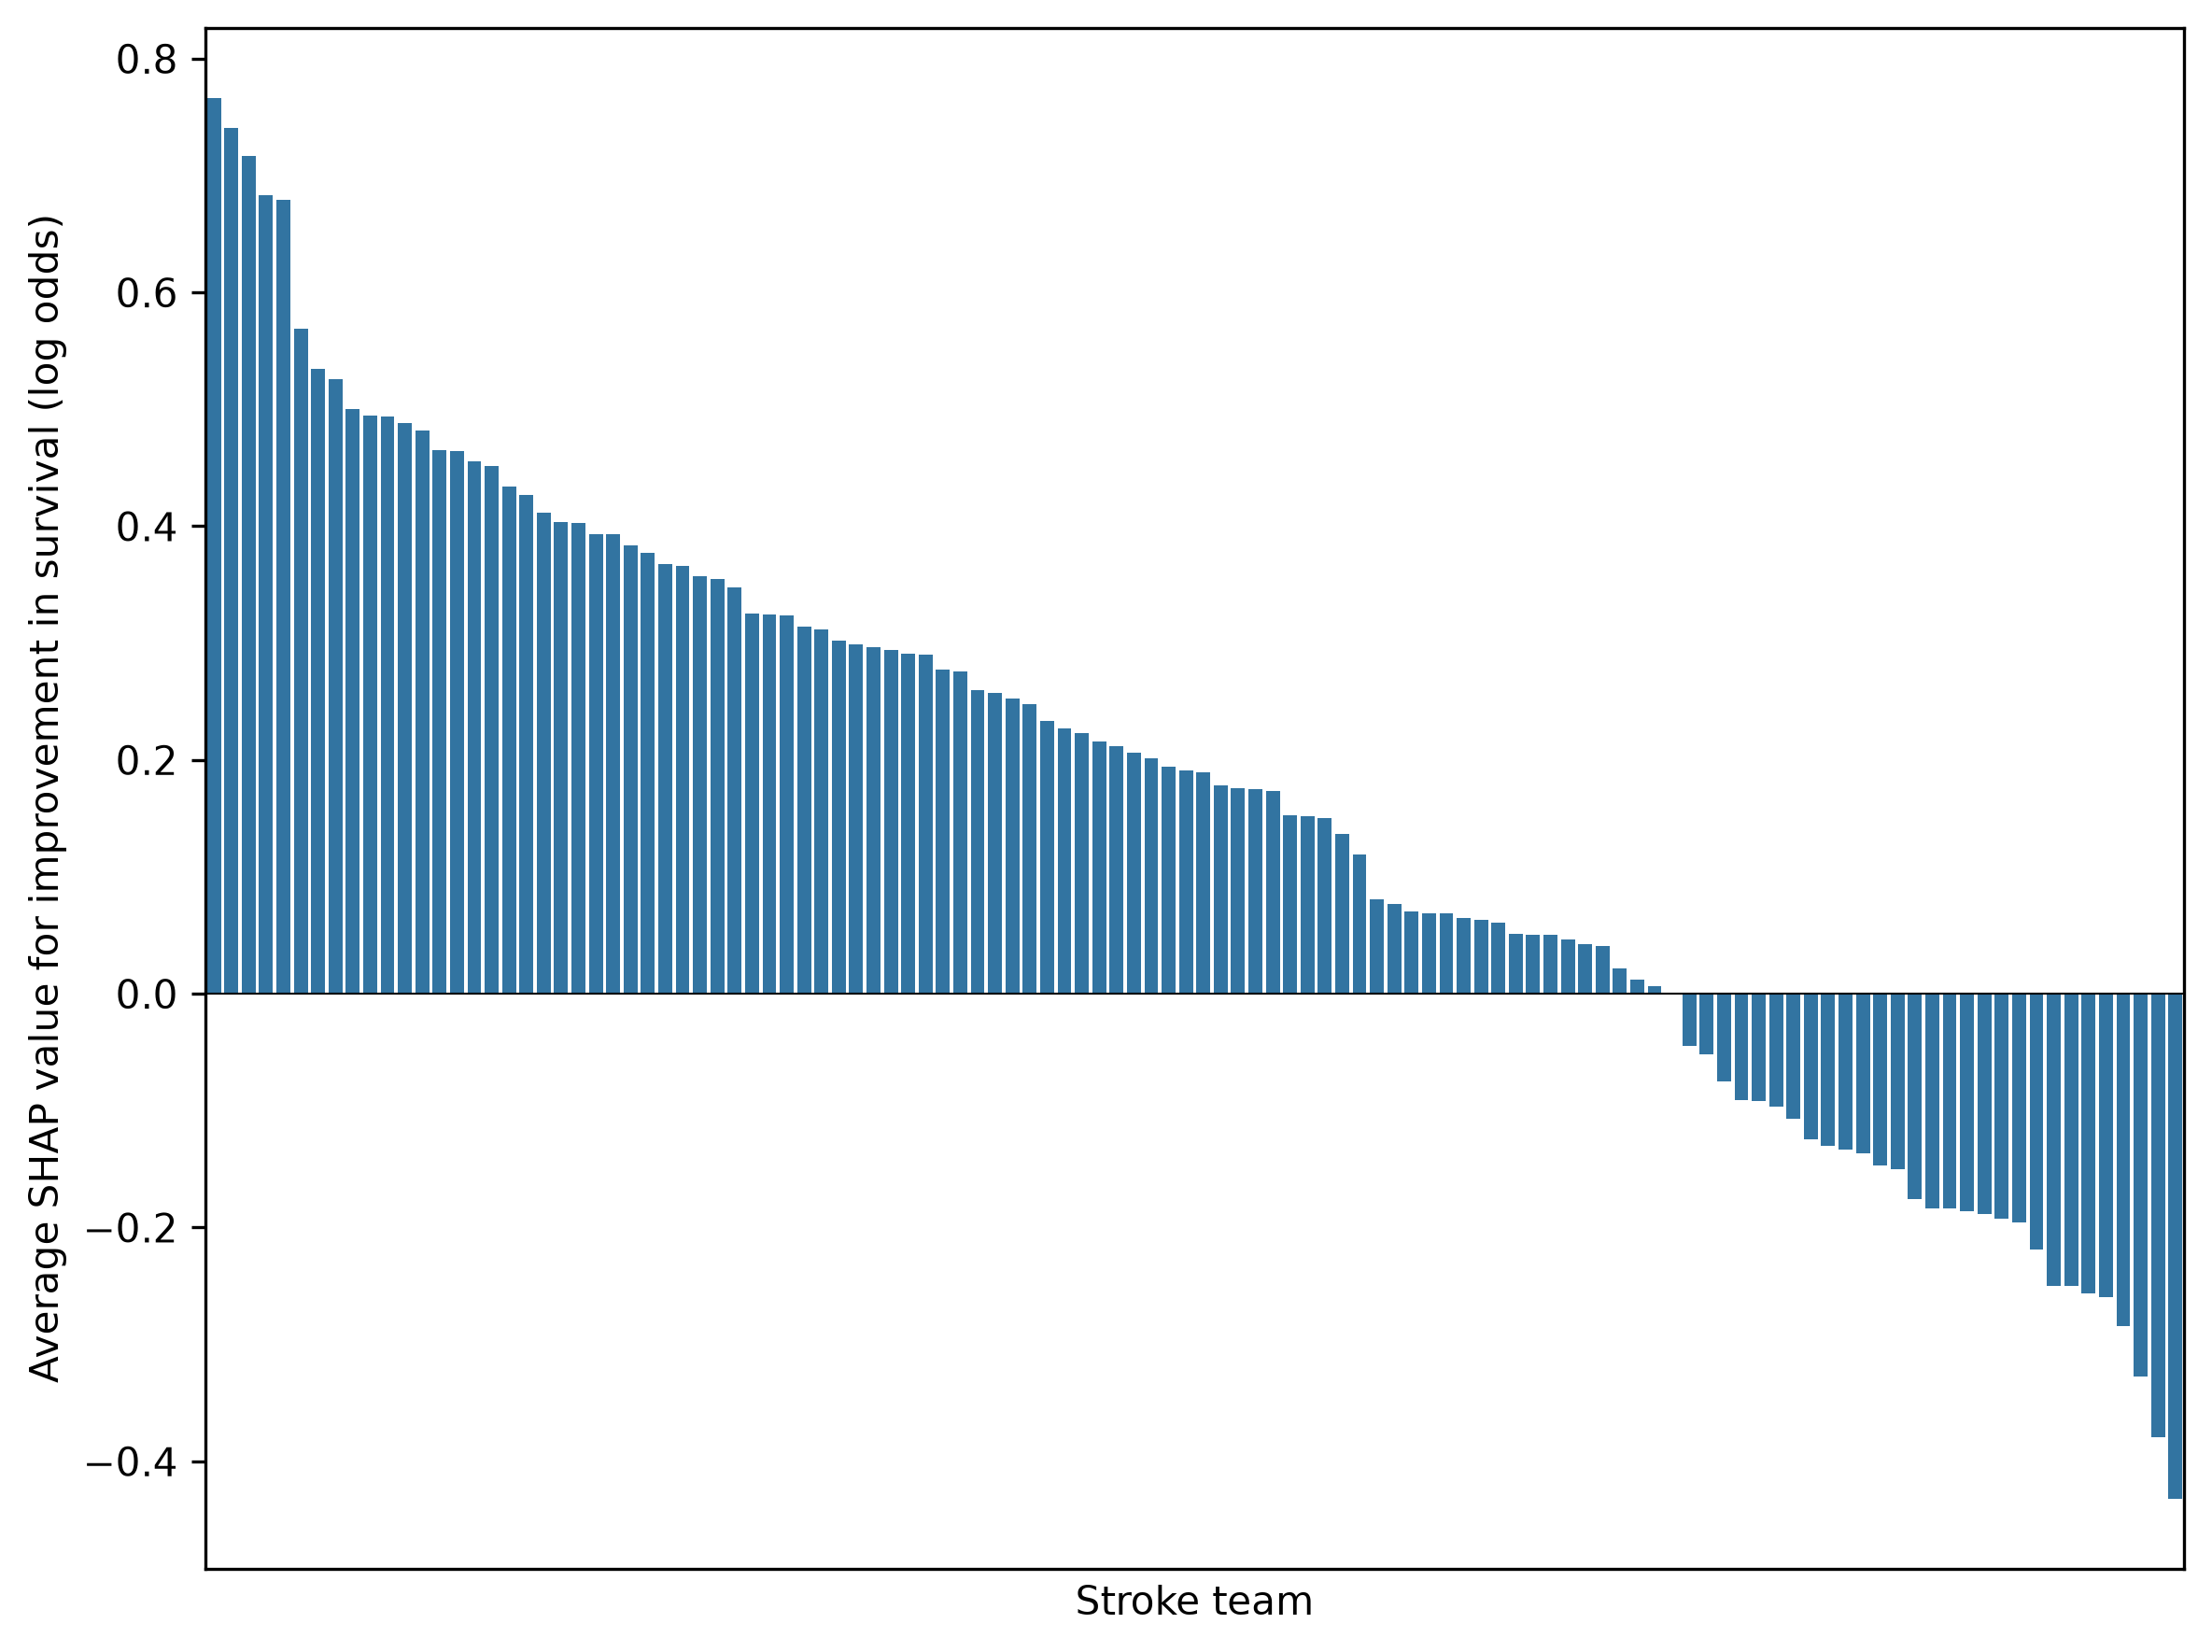
\includegraphics[width=\linewidth]{images/shap/shap_all_patients_survival_stroke_team.png}
        %\caption{}
        \label{fig:bottom-right}
    \end{subfigure}

    \caption{SHAP analysis of feature contributions to predicting survival in stroke patients. \textit{Top}: A SHAP summary plot detailing the impact of features on the model's log-odds predictions. Each point represents an individual patient instance. The position on the x-axis indicates the SHAP value, where positive values increase the predicted odds of survival, and negative values decrease it. For continuous and binary variables, colour represents the original feature value (red indicating high values; blue indicating low values). Categorical variables (\textit{stroke team} and \textit{ethnicity}) are plotted in grey. \textit{Bottom left}: Violin plots illustrating the distribution of SHAP values across distinct ethnic groups. This panel highlights the marginal impact and variance of ethnicity on the model’s prediction for survival. \textit{Bottom Right}: A ranked bar chart displaying the average SHAP value associated with each individual stroke team. This panel visualizes institutional variation, reflecting the contribution of the treating stroke team to the predicted survival outcome after accounting for patient-level clinical characteristics.}
    \label{fig:shap_survival_all}
\end{figure}

%% Untreated patients

\begin{figure}[htbp]
    \centering
    
    % Top image (Full width)
    \begin{subfigure}{0.50\textwidth}
        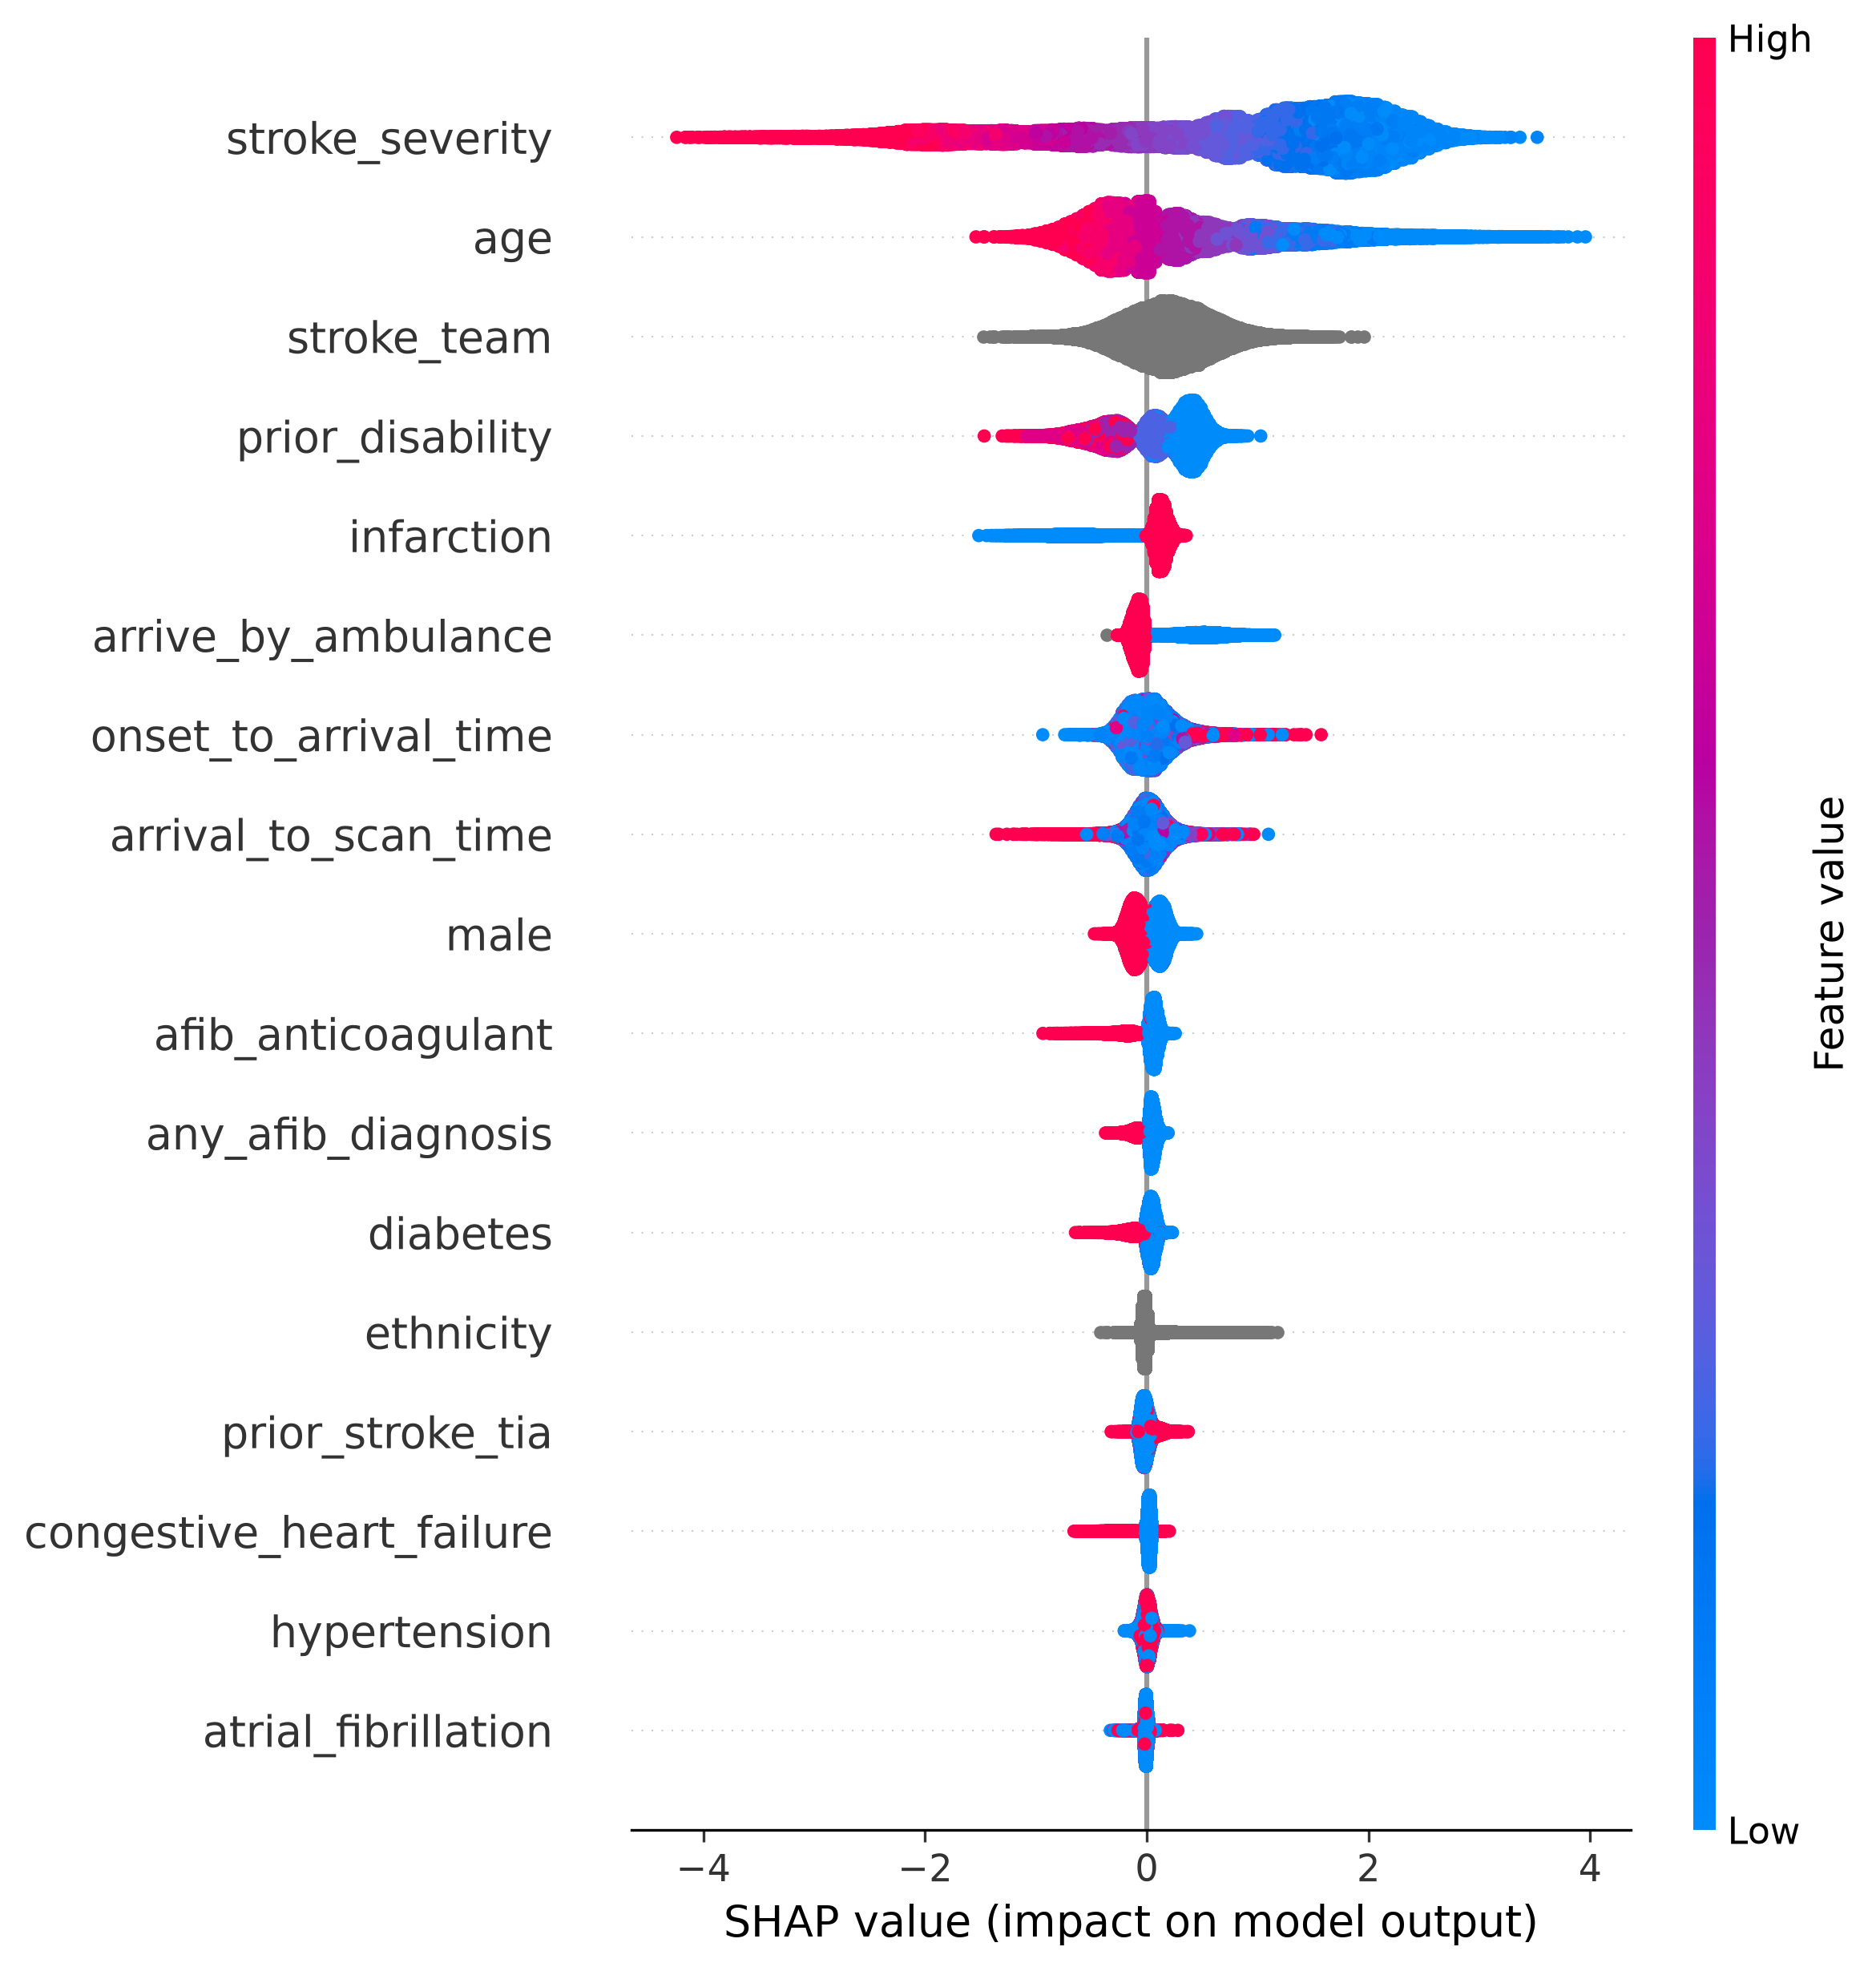
\includegraphics[width=\linewidth]{images/shap/shap_untreated_patients_survival.png}
        %\caption{}
        \label{fig:top}
    \end{subfigure}

    \vspace{0.5cm} % Optional vertical space between rows

    % Bottom left image (~45% width)
    \begin{subfigure}{0.407\textwidth}
        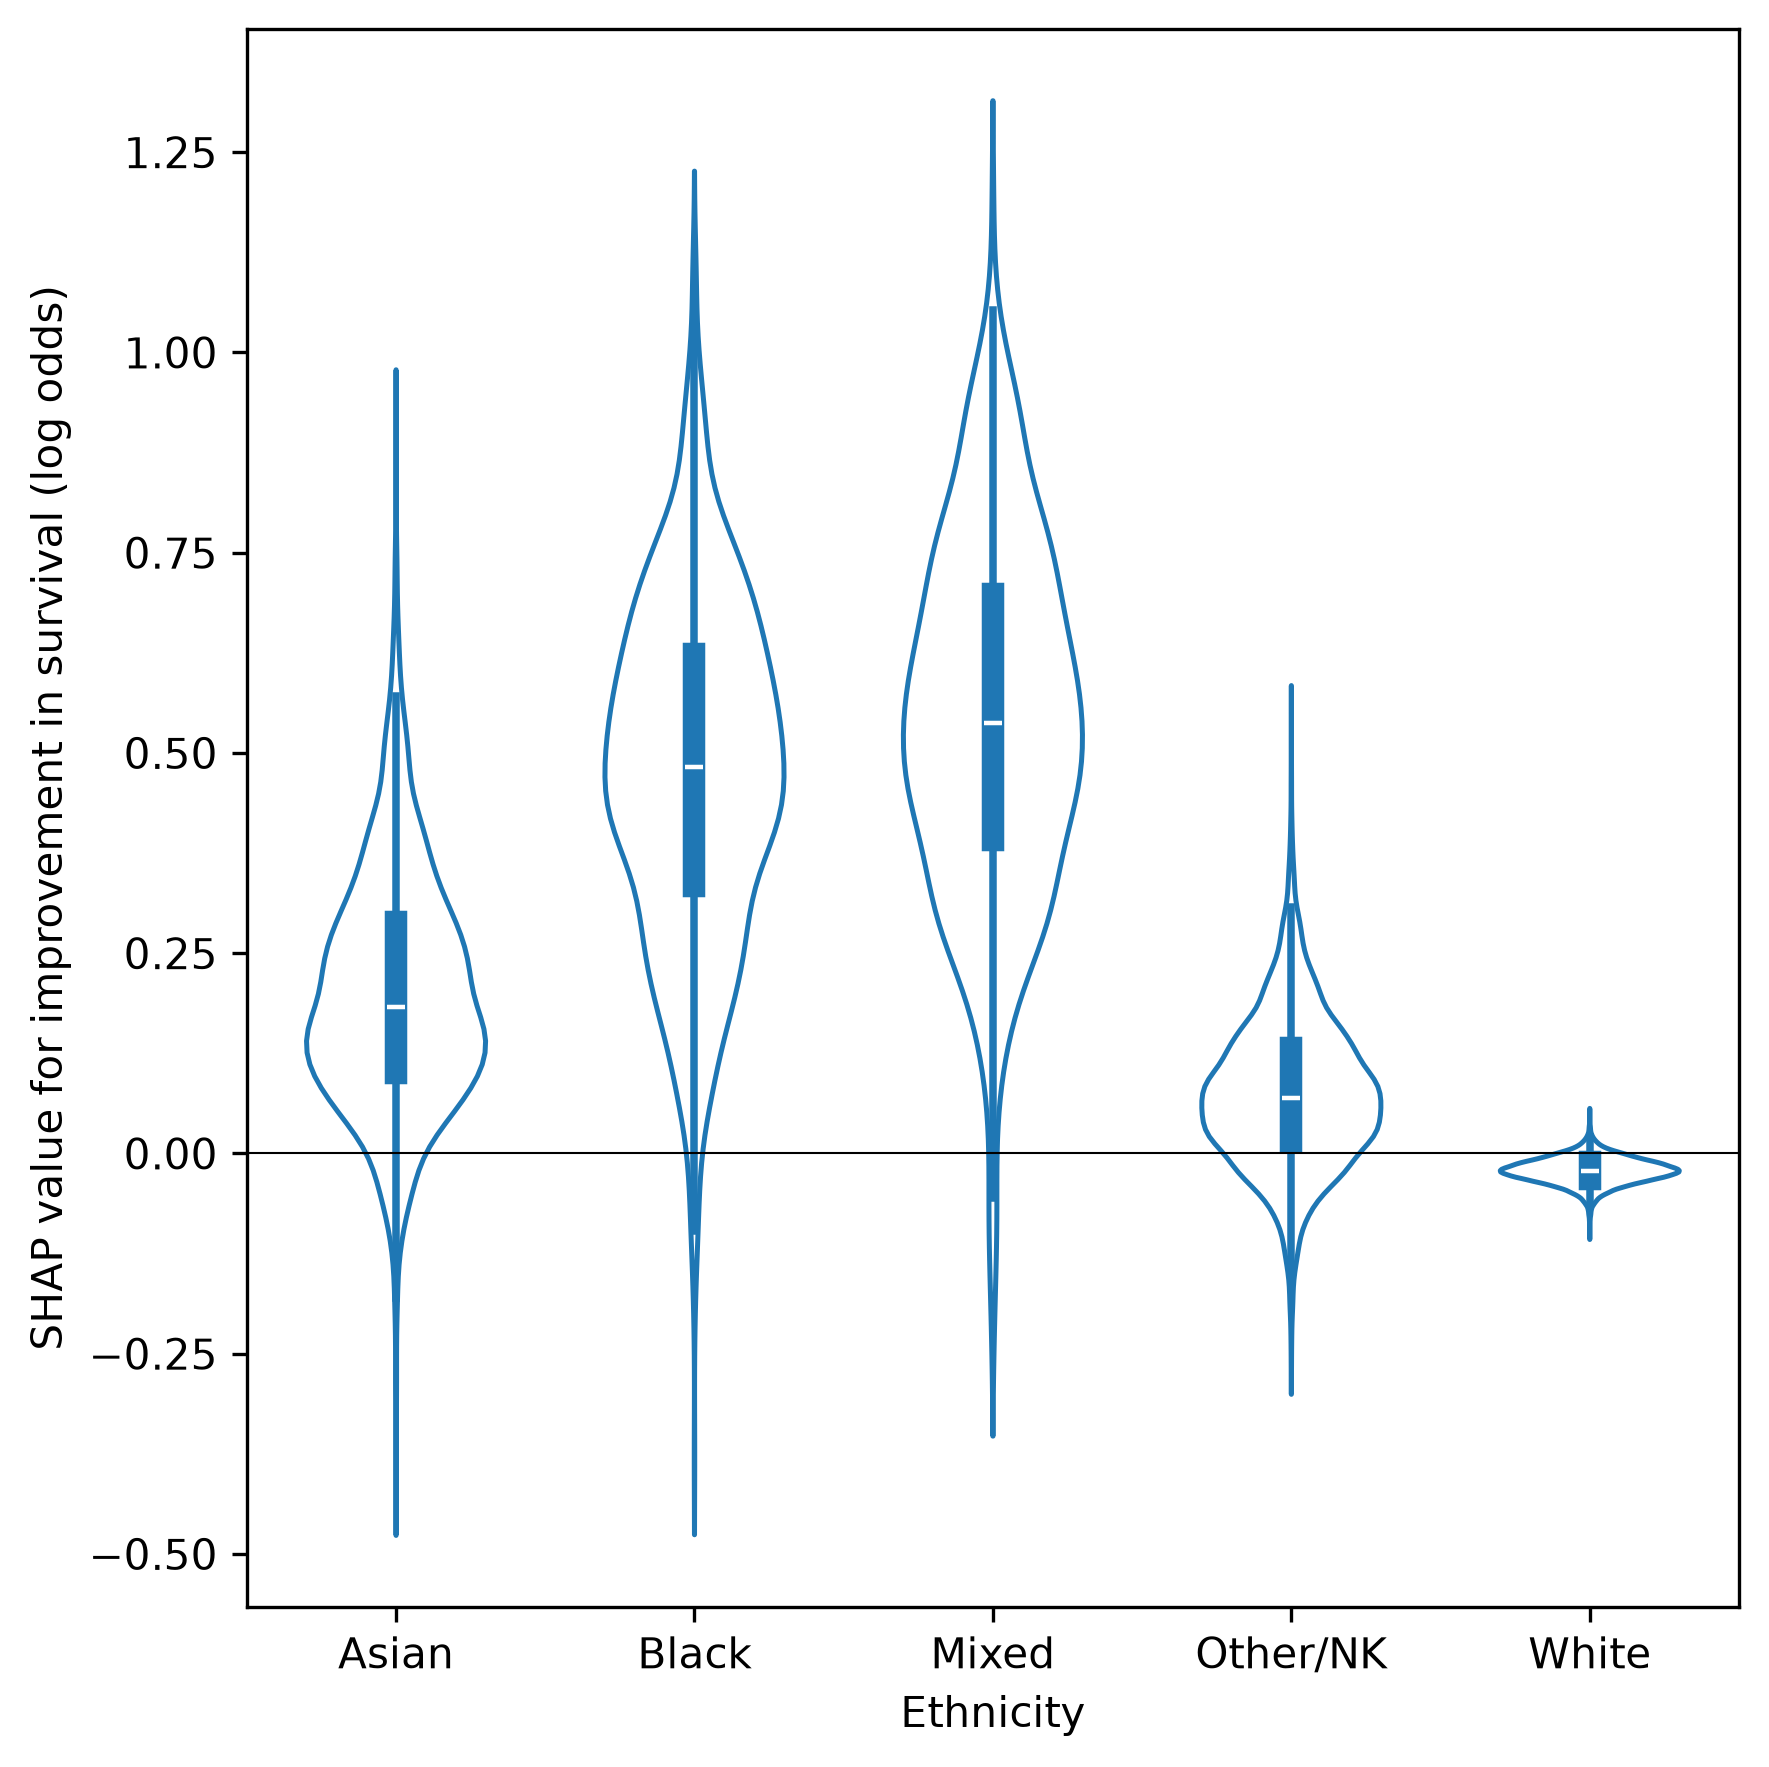
\includegraphics[width=\linewidth]{images/shap/shap_untreated_patients_survival_ethnicity.png}
        %\caption{}
        \label{fig:bottom-left}
    \end{subfigure}
    \hfill % Adds flexible horizontal spacing
    % Bottom right image (~55% width)
    \begin{subfigure}{0.543\textwidth}
        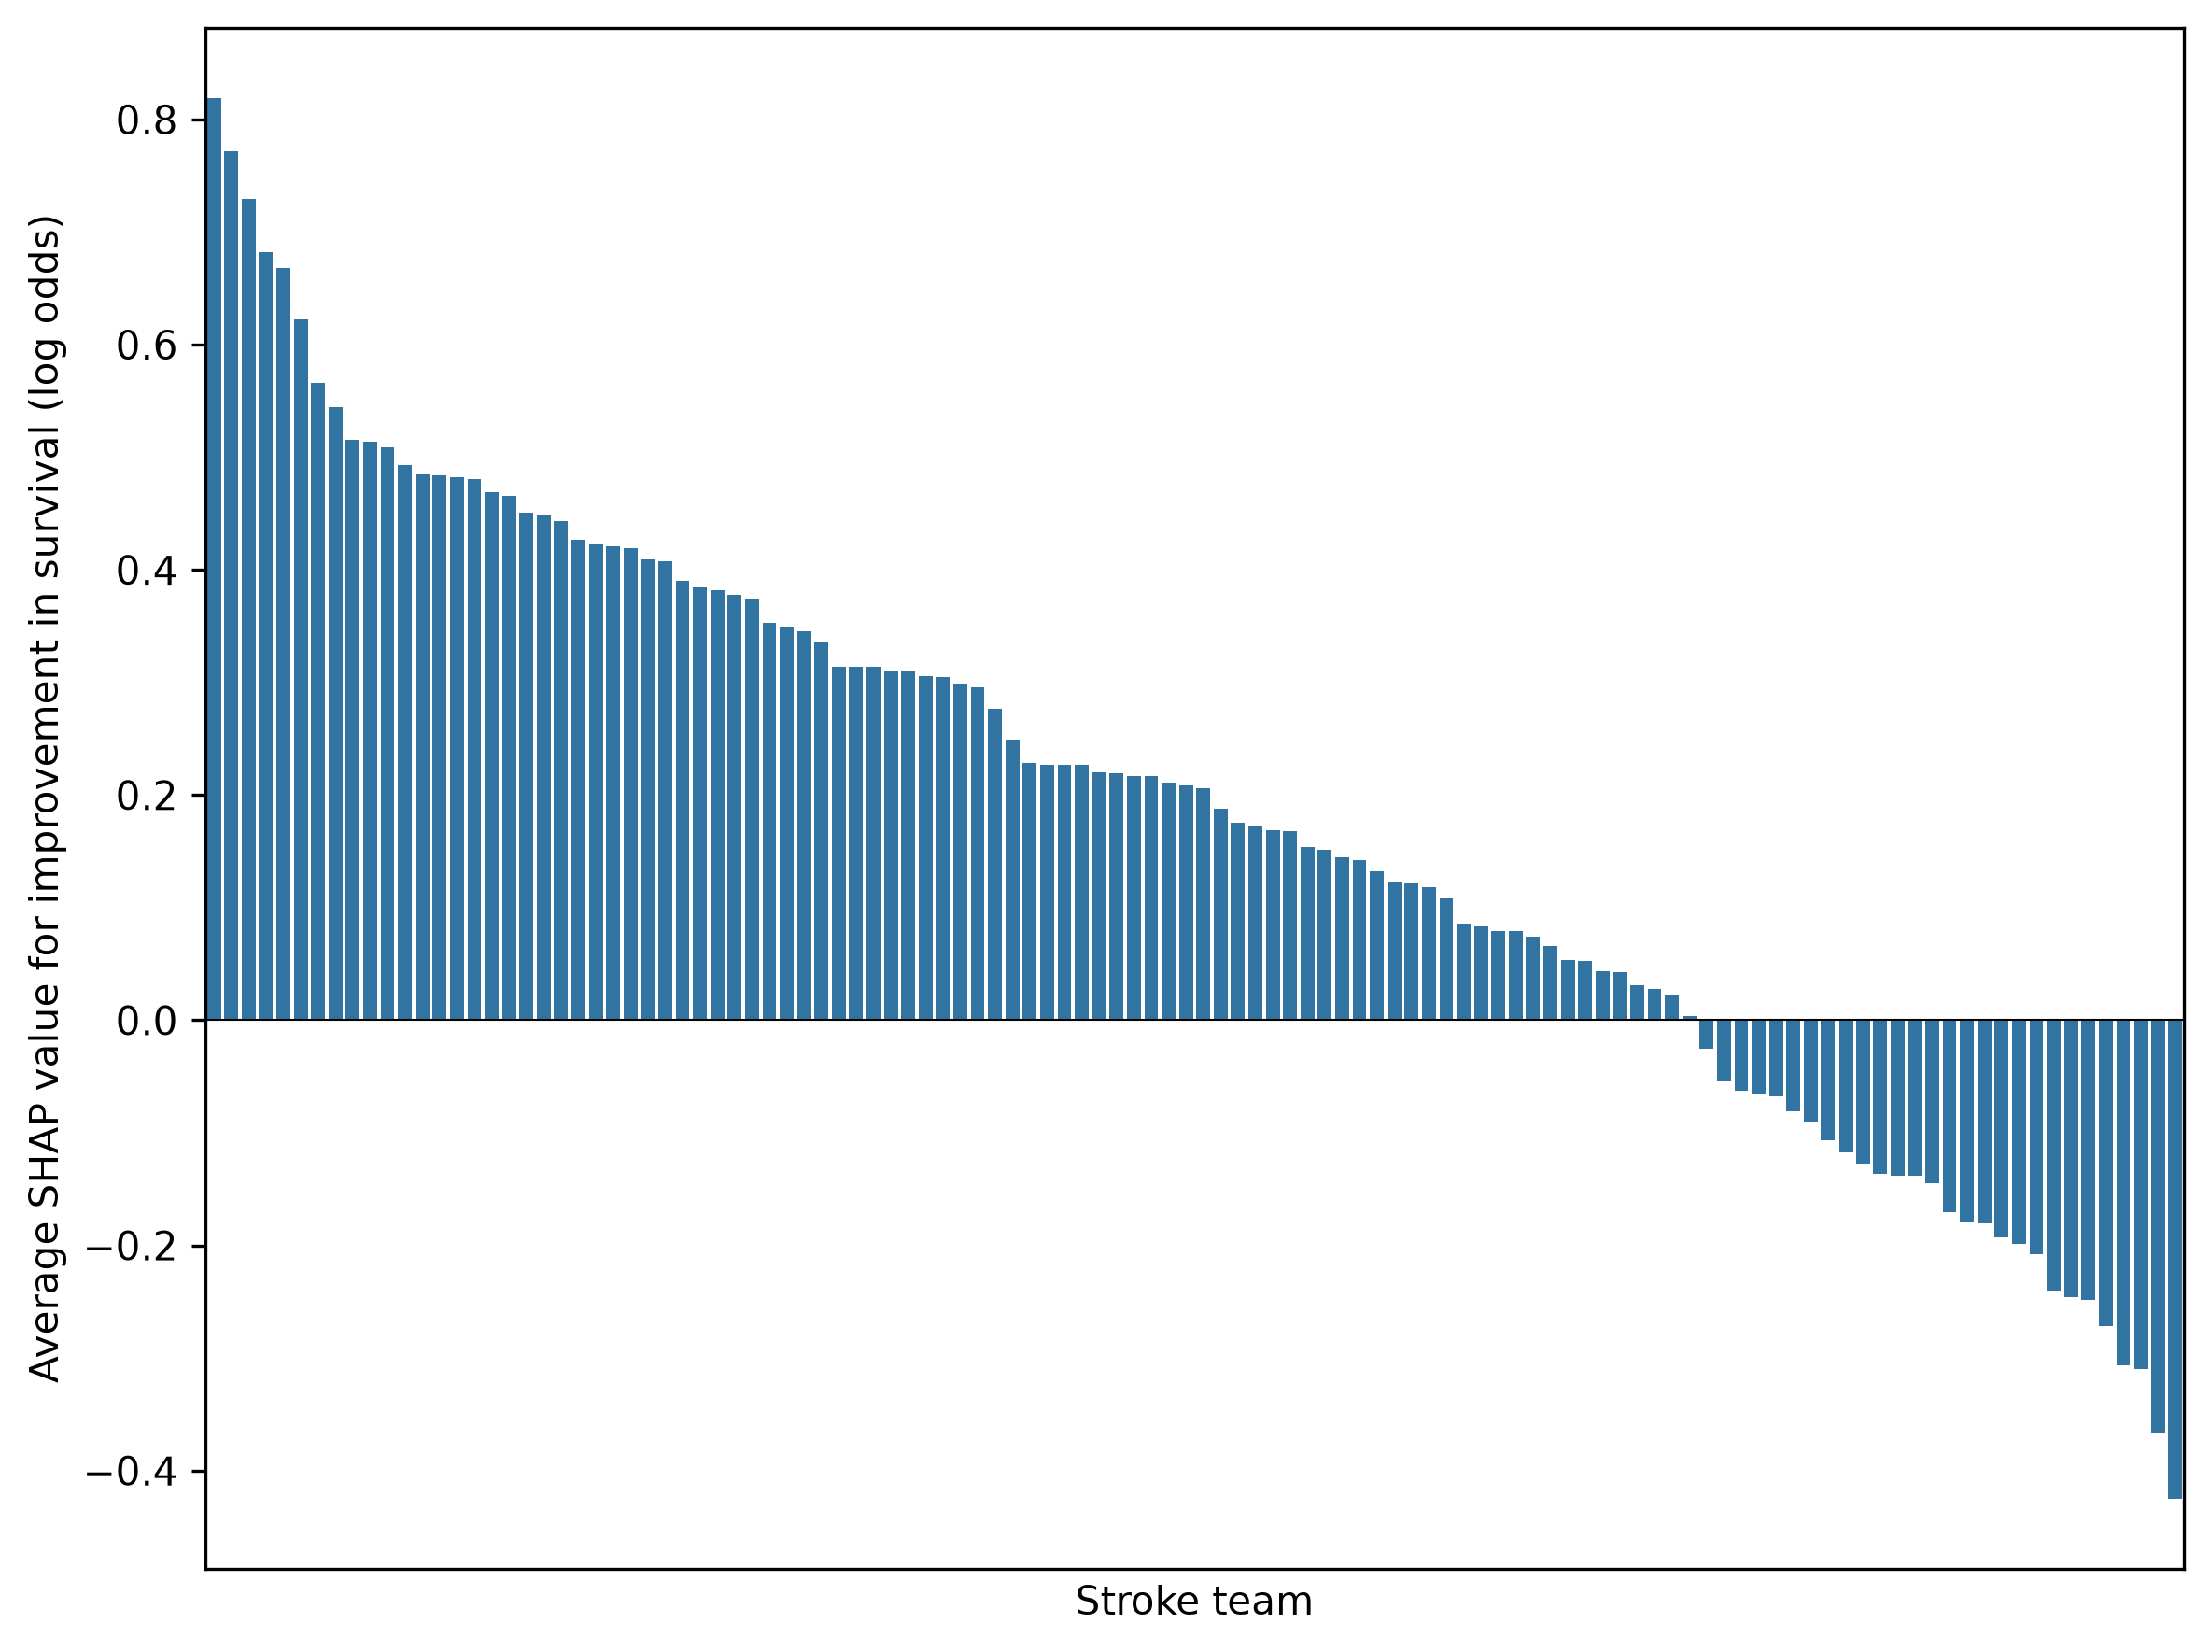
\includegraphics[width=\linewidth]{images/shap/shap_untreated_patients_survival_stroke_team.png}
        %\caption{}
        \label{fig:bottom-right}
    \end{subfigure}

    \caption{SHAP analysis of feature contributions to predicting survival in stroke patients who did not receive thrombolysis or thrombectomy. \textit{Top}: A SHAP summary plot detailing the impact of features on the model's log-odds predictions. Each point represents an individual patient instance. The position on the x-axis indicates the SHAP value, where positive values increase the predicted odds of survival, and negative values decrease it. For continuous and binary variables, colour represents the original feature value (red indicating high values; blue indicating low values). Categorical variables (\textit{stroke team} and \textit{ethnicity}) are plotted in grey. \textit{Bottom left}: Violin plots illustrating the distribution of SHAP values across distinct ethnic groups. This panel highlights the marginal impact and variance of ethnicity on the model’s prediction for survival. \textit{Bottom Right}: A ranked bar chart displaying the average SHAP value associated with each individual stroke team. This panel visualizes institutional variation, reflecting the contribution of the treating stroke team to the predicted survival outcome after accounting for patient-level clinical characteristics.}
    \label{fig:shap_survival_all}
\end{figure}